\documentclass[11pt]{article}
\usepackage[margin=1in]{geometry}
\usepackage{amsmath,amssymb,booktabs,graphicx,xcolor,natbib,microtype,tikz,rotating,placeins,multirow}
\renewcommand{\topfraction}{0.9}\renewcommand{\textfraction}{0.07}\renewcommand{\floatpagefraction}{0.75}
\usetikzlibrary{positioning,calc}
\usepackage{times}
\usepackage[colorlinks=true,linkcolor=blue!60!black,citecolor=blue!60!black,urlcolor=blue!60!black,pdftitle={PALIMPSEST: Evaluating Retraction and Uncertainty in LLM Memory},pdfauthor={Christian Leiva Beltran}]{hyperref}
\newcommand{\pal}{\textsc{Palimpsest}}
\newcommand{\rs}{\textsc{Revise-Stream}}
\newcommand{\sOnePropEffect}{20.6}
\newcommand{\sOnePropLo}{18.7}
\newcommand{\sOnePropHi}{22.5}
\newcommand{\sOnePropN}{495}
\newcommand{\sOneCommitUnsup}{9.0}
\newcommand{\sOneCommitUnsupLo}{7.8}
\newcommand{\sOneCommitUnsupHi}{10.2}
\newcommand{\sOneCommitRate}{78}
\newcommand{\sOneAbstainRes}{0.000}
\newcommand{\sOneAbstainUnres}{0.393}
\newcommand{\sOneCommitRes}{0.770}
\newcommand{\sOneCommitUnres}{0.000}
\newcommand{\sOneTdbWarr}{19.3}
\newcommand{\sOneTdbCommit}{85}
\newcommand{\sOneProvP}{0.99}
\newcommand{\sOneProvR}{0.99}
\newcommand{\sOneWarrPerStream}{7.4}
\newcommand{\sOneAnswers}{16683}
\newcommand{\sOneLitPZeroEffect}{36.2}
\newcommand{\sOneLitPZeroWarr}{3.4}
\newcommand{\sOnePOneEffect}{31.2}
\newcommand{\sOnePOneWarr}{3.5}
\newcommand{\RqLearnedEce}{0.113}
\newcommand{\RqLearnedBrier}{0.175}
\newcommand{\RqLearnedAurc}{0.131}
\newcommand{\RqPriorEce}{0.227}
\newcommand{\RqPriorBrier}{0.255}
\newcommand{\RqPriorAurc}{0.168}
\newcommand{\RqLogregEce}{0.034}
\newcommand{\RqLogregBrier}{0.138}
\newcommand{\RqLogregAurc}{0.112}
\newcommand{\RqDefaultEce}{0.118}
\newcommand{\RqDefaultBrier}{0.182}
\newcommand{\RqDefaultAurc}{0.138}
\newcommand{\RqNoRecEce}{0.202}
\newcommand{\RqNoRecBrier}{0.236}
\newcommand{\RqNoRecAurc}{0.156}
\newcommand{\RqNoOrigEce}{0.121}
\newcommand{\RqNoOrigBrier}{0.179}
\newcommand{\RqNoOrigAurc}{0.136}
\newcommand{\RqN}{2481}
\newcommand{\PoisHarmPal}{11.2}
\newcommand{\PoisHarmTdb}{15.1}
\newcommand{\PoisHarmCommit}{13.7}
\newcommand{\PoisSupLowPois}{0.21--0.33}
\newcommand{\PoisSupLowHon}{0.65--0.67}
\newcommand{\PoisSupTrPois}{0.63--0.66}
\newcommand{\PoisSupTrHon}{0.63--0.67}
\newcommand{\sTwoHOne}{44.2}
\newcommand{\sTwoHOneLo}{39.0}
\newcommand{\sTwoHOneHi}{49.7}
\newcommand{\sTwoHOneN}{99}
\newcommand{\sTwoProp}{20.7}
\newcommand{\sTwoPropLo}{16.2}
\newcommand{\sTwoPropHi}{25.4}
\newcommand{\sTwoPalWarr}{0.956}
\newcommand{\sTwoPalRes}{0.976}
\newcommand{\sTwoPalUnres}{0.834}
\newcommand{\sTwoPalCommit}{0.080}
\newcommand{\sTwoPalUnsup}{0.083}
\newcommand{\sTwoPalCost}{0.078}
\newcommand{\sTwoPalTok}{188}
\newcommand{\sTwoLogWarr}{0.514}
\newcommand{\sTwoLogRes}{0.666}
\newcommand{\sTwoLogUnres}{0.128}
\newcommand{\sTwoLogCommit}{0.572}
\newcommand{\sTwoLogUnsup}{0.392}
\newcommand{\sTwoLogCost}{0.234}
\newcommand{\sTwoLogTok}{532}
\newcommand{\sTwoNlWarr}{0.330}
\newcommand{\sTwoNlRes}{0.554}
\newcommand{\sTwoNlUnres}{0.101}
\newcommand{\sTwoNlCommit}{0.606}
\newcommand{\sTwoNlUnsup}{0.456}
\newcommand{\sTwoNlCost}{0.203}
\newcommand{\sTwoNlTok}{439}
\newcommand{\sTwoTdbWarr}{0.779}
\newcommand{\sTwoTdbRes}{0.895}
\newcommand{\sTwoTdbUnres}{0.000}
\newcommand{\sTwoTdbCommit}{0.837}
\newcommand{\sTwoTdbUnsup}{0.142}
\newcommand{\sTwoTdbCost}{0.078}
\newcommand{\sTwoTdbTok}{188}
\newcommand{\sTwoCommitWarr}{0.979}
\newcommand{\sTwoCommitRes}{0.987}
\newcommand{\sTwoCommitUnres}{0.045}
\newcommand{\sTwoCommitCommit}{0.758}
\newcommand{\sTwoCommitUnsup}{0.104}
\newcommand{\sTwoCommitCost}{0.078}
\newcommand{\sTwoCommitTok}{188}
\newcommand{\sTwoTopkWarr}{0.419}
\newcommand{\sTwoTopkRes}{0.614}
\newcommand{\sTwoTopkUnres}{0.103}
\newcommand{\sTwoTopkCommit}{0.504}
\newcommand{\sTwoTopkUnsup}{0.533}
\newcommand{\sTwoTopkCost}{0.196}
\newcommand{\sTwoTopkTok}{454}
\newcommand{\sTwoNopropWarr}{0.749}
\newcommand{\sTwoNopropRes}{0.920}
\newcommand{\sTwoNopropUnres}{0.813}
\newcommand{\sTwoNopropCommit}{0.079}
\newcommand{\sTwoNopropUnsup}{0.093}
\newcommand{\sTwoNopropCost}{0.078}
\newcommand{\sTwoNopropTok}{188}
\newcommand{\sTwoRuleWarr}{0.956}
\newcommand{\sTwoRuleRes}{0.976}
\newcommand{\sTwoRuleUnres}{0.834}
\newcommand{\sTwoRuleCommit}{0.080}
\newcommand{\sTwoRuleUnsup}{0.083}
\newcommand{\sTwoRuleCost}{0.078}
\newcommand{\sTwoRuleTok}{188}
\newcommand{\sTwoExtSlot}{1.5}
\newcommand{\sTwoExtMissed}{3.7}
\newcommand{\sTwoExtSpur}{0.0}
\newcommand{\sTwoExtValid}{6.0}
\newcommand{\sTwoExtFail}{0.1}
\newcommand{\sTwoWarrPerStream}{7.41}
\newcommand{\sTwoSubPalWarr}{0.989}
\newcommand{\sTwoSubN}{30}
\newcommand{\sTwoCtwoLogWarr}{0.400}
\newcommand{\sTwoCtwoLogDirect}{0.703}
\newcommand{\sTwoCtwoLogRes}{0.607}
\newcommand{\sTwoCtwoLogUnres}{0.134}
\newcommand{\sTwoCtwoLogCommit}{0.533}
\newcommand{\sTwoCtwoLogMalformed}{0.000}
\newcommand{\sTwoCtwoLogTok}{552}
\newcommand{\sTwoCtwoLogCost}{0.243}
\newcommand{\sTwoCtwoLogDiff}{59.0}
\newcommand{\sTwoCtwoLogDiffLo}{51.4}
\newcommand{\sTwoCtwoLogDiffHi}{66.5}
\newcommand{\sTwoCtwoLogDiffN}{30}
\newcommand{\sTwoCtwoTopTenWarr}{0.225}
\newcommand{\sTwoCtwoTopTenDirect}{0.787}
\newcommand{\sTwoCtwoTopTenRes}{0.572}
\newcommand{\sTwoCtwoTopTenUnres}{0.138}
\newcommand{\sTwoCtwoTopTenCommit}{0.377}
\newcommand{\sTwoCtwoTopTenMalformed}{0.000}
\newcommand{\sTwoCtwoTopTenTok}{399}
\newcommand{\sTwoCtwoTopTenCost}{0.171}
\newcommand{\sTwoCtwoTopTenDiff}{76.5}
\newcommand{\sTwoCtwoTopTenDiffLo}{69.6}
\newcommand{\sTwoCtwoTopTenDiffHi}{82.7}
\newcommand{\sTwoCtwoTopTenDiffN}{30}
\newcommand{\sTwoCtwoTopTwentyWarr}{0.385}
\newcommand{\sTwoCtwoTopTwentyDirect}{0.723}
\newcommand{\sTwoCtwoTopTwentyRes}{0.610}
\newcommand{\sTwoCtwoTopTwentyUnres}{0.136}
\newcommand{\sTwoCtwoTopTwentyCommit}{0.412}
\newcommand{\sTwoCtwoTopTwentyMalformed}{0.000}
\newcommand{\sTwoCtwoTopTwentyTok}{424}
\newcommand{\sTwoCtwoTopTwentyCost}{0.182}
\newcommand{\sTwoCtwoTopTwentyDiff}{60.4}
\newcommand{\sTwoCtwoTopTwentyDiffLo}{51.4}
\newcommand{\sTwoCtwoTopTwentyDiffHi}{69.3}
\newcommand{\sTwoCtwoTopTwentyDiffN}{30}
\newcommand{\sTwoCtwoTopFortyWarr}{0.429}
\newcommand{\sTwoCtwoTopFortyDirect}{0.739}
\newcommand{\sTwoCtwoTopFortyRes}{0.628}
\newcommand{\sTwoCtwoTopFortyUnres}{0.133}
\newcommand{\sTwoCtwoTopFortyCommit}{0.471}
\newcommand{\sTwoCtwoTopFortyMalformed}{0.000}
\newcommand{\sTwoCtwoTopFortyTok}{464}
\newcommand{\sTwoCtwoTopFortyCost}{0.201}
\newcommand{\sTwoCtwoTopFortyDiff}{56.0}
\newcommand{\sTwoCtwoTopFortyDiffLo}{45.7}
\newcommand{\sTwoCtwoTopFortyDiffHi}{66.2}
\newcommand{\sTwoCtwoTopFortyDiffN}{30}
\newcommand{\sTwoCtwoNlWarr}{0.323}
\newcommand{\sTwoCtwoNlDirect}{0.672}
\newcommand{\sTwoCtwoNlRes}{0.524}
\newcommand{\sTwoCtwoNlUnres}{0.102}
\newcommand{\sTwoCtwoNlCommit}{0.563}
\newcommand{\sTwoCtwoNlMalformed}{0.000}
\newcommand{\sTwoCtwoNlTok}{448}
\newcommand{\sTwoCtwoNlCost}{0.207}
\newcommand{\sTwoCtwoNlDiff}{66.7}
\newcommand{\sTwoCtwoNlDiffLo}{56.5}
\newcommand{\sTwoCtwoNlDiffHi}{76.2}
\newcommand{\sTwoCtwoNlDiffN}{30}
\newcommand{\sTwoSubTopFortyWarr}{0.419}
\newcommand{\sTwoSubTopFortyDirect}{0.731}
\newcommand{\sTwoSubTopFortyRes}{0.614}
\newcommand{\sTwoSubTopFortyUnres}{0.103}
\newcommand{\sTwoSubTopFortyCommit}{0.504}
\newcommand{\sTwoSubTopFortyMalformed}{0.000}
\newcommand{\sTwoSubTopFortyTok}{454}
\newcommand{\sTwoSubTopFortyCost}{0.196}
\newcommand{\sTwoSubTopFortyDiff}{57.0}
\newcommand{\sTwoSubTopFortyDiffLo}{46.8}
\newcommand{\sTwoSubTopFortyDiffHi}{67.1}
\newcommand{\sTwoSubTopFortyDiffN}{30}
\newcommand{\sTwoSubNlWarr}{0.330}
\newcommand{\sTwoSubNlDirect}{0.685}
\newcommand{\sTwoSubNlRes}{0.554}
\newcommand{\sTwoSubNlUnres}{0.101}
\newcommand{\sTwoSubNlCommit}{0.606}
\newcommand{\sTwoSubNlMalformed}{0.000}
\newcommand{\sTwoSubNlTok}{439}
\newcommand{\sTwoSubNlCost}{0.203}
\newcommand{\sTwoSubNlDiff}{66.0}
\newcommand{\sTwoSubNlDiffLo}{55.8}
\newcommand{\sTwoSubNlDiffHi}{75.3}
\newcommand{\sTwoSubNlDiffN}{30}
\newcommand{\sTwoSubLogDiff}{58.2}
\newcommand{\sTwoSubLogDiffLo}{50.5}
\newcommand{\sTwoSubLogDiffHi}{66.3}
\newcommand{\sTwoSubLogWarr}{0.408}
\newcommand{\sThreeCtwoLogWarr}{0.019}
\newcommand{\sThreeCtwoLogDirect}{0.491}
\newcommand{\sThreeCtwoLogRes}{0.205}
\newcommand{\sThreeCtwoLogUnres}{0.394}
\newcommand{\sThreeCtwoLogCommit}{0.485}
\newcommand{\sThreeCtwoNlWarr}{0.173}
\newcommand{\sThreeCtwoNlDirect}{0.466}
\newcommand{\sThreeCtwoNlRes}{0.208}
\newcommand{\sThreeCtwoNlUnres}{0.318}
\newcommand{\sThreeCtwoNlCommit}{0.439}
\newcommand{\sStrongHOne}{18.7}
\newcommand{\sStrongHOneLo}{7.4}
\newcommand{\sStrongHOneHi}{33.1}
\newcommand{\sStrongPalWarr}{1.000}
\newcommand{\sStrongLogWarr}{0.813}
\newcommand{\sStrongLogCommit}{0.489}
\newcommand{\sStrongExtSlot}{0.3}
\newcommand{\xE}{188}
\newcommand{\xAnl}{6.5}
\newcommand{\xAlog}{5.1}
\newcommand{\xRstar}{0.22}
\newcommand{\xNobs}{131}
\newcommand{\RqTwoSupEce}{0.150}
\newcommand{\RqTwoSupBrier}{0.133}
\newcommand{\RqTwoSupAurc}{0.073}
\newcommand{\RqTwoSupN}{973}
\newcommand{\RqTwoVerbEce}{0.088}
\newcommand{\RqTwoVerbBrier}{0.091}
\newcommand{\RqTwoVerbAurc}{0.069}
\newcommand{\RqTwoVerbN}{973}
\newcommand{\RqTwoSampEce}{0.073}
\newcommand{\RqTwoSampBrier}{0.083}
\newcommand{\RqTwoSampAurc}{0.078}
\newcommand{\RqTwoSampN}{300}
\newcommand{\nzSlotTwentyPal}{0.449}
\newcommand{\nzSlotTwentyTdb}{0.388}
\newcommand{\nzSlotThirtyfivePal}{0.273}
\newcommand{\nzSlotThirtyfiveTdb}{0.301}
\newcommand{\nzCueFiftyPal}{0.562}
\newcommand{\nzCueFiftyTdb}{0.758}
\newcommand{\sThreeHOne}{90.4}
\newcommand{\sThreeHOneLo}{73.1}
\newcommand{\sThreeHOneHi}{100.0}
\newcommand{\sThreeHOneN}{13}
\newcommand{\sThreeProp}{19.9}
\newcommand{\sThreePropLo}{2.6}
\newcommand{\sThreePropHi}{41.0}
\newcommand{\sThreeDirect}{45.7}
\newcommand{\sThreeDirectLo}{31.1}
\newcommand{\sThreeDirectHi}{60.5}
\newcommand{\sThreeDirectN}{27}
\newcommand{\sThreePalWarr}{0.923}
\newcommand{\sThreePalDirect}{0.976}
\newcommand{\sThreePalRes}{0.978}
\newcommand{\sThreePalUnres}{0.909}
\newcommand{\sThreePalCommit}{0.000}
\newcommand{\sThreePalUnsup}{0.107}
\newcommand{\sThreeLogWarr}{0.019}
\newcommand{\sThreeLogDirect}{0.519}
\newcommand{\sThreeLogRes}{0.185}
\newcommand{\sThreeLogUnres}{0.333}
\newcommand{\sThreeLogCommit}{0.545}
\newcommand{\sThreeLogUnsup}{0.476}
\newcommand{\sThreeTdbWarr}{0.865}
\newcommand{\sThreeTdbDirect}{0.884}
\newcommand{\sThreeTdbRes}{0.692}
\newcommand{\sThreeTdbUnres}{0.000}
\newcommand{\sThreeTdbCommit}{1.000}
\newcommand{\sThreeTdbUnsup}{0.107}
\newcommand{\sThreeRuleWarr}{0.923}
\newcommand{\sThreeRuleDirect}{0.976}
\newcommand{\sThreeRuleRes}{0.978}
\newcommand{\sThreeRuleUnres}{0.909}
\newcommand{\sThreeRuleCommit}{0.000}
\newcommand{\sThreeRuleUnsup}{0.107}
\newcommand{\sThreeCommitWarr}{0.923}
\newcommand{\sThreeCommitDirect}{0.976}
\newcommand{\sThreeCommitRes}{0.978}
\newcommand{\sThreeCommitUnres}{0.000}
\newcommand{\sThreeCommitCommit}{1.000}
\newcommand{\sThreeCommitUnsup}{0.107}
\newcommand{\sThreeNlWarr}{0.077}
\newcommand{\sThreeNlDirect}{0.451}
\newcommand{\sThreeNlRes}{0.181}
\newcommand{\sThreeNlUnres}{0.182}
\newcommand{\sThreeNlCommit}{0.576}
\newcommand{\sThreeNlUnsup}{0.446}
\newcommand{\sThreeExtSlot}{1.2}
\newcommand{\sThreeExtMissed}{0.0}
\newcommand{\sThreeExtSpur}{0.0}
\newcommand{\sThreeExtFail}{0.1}
\newcommand{\sThreeWarrPerStream}{0.80}
\newcommand{\sThreeEstTotal}{338}
\newcommand{\sThreeEstEmpty}{94}
\newcommand{\sThreeHoldsFalse}{102}
\newcommand{\sThreeWarrEmpty}{3}
\newcommand{\sThreeWarrTotal}{24}
\newcommand{\sThreePalResNe}{0.954}
\newcommand{\sThreePalWarrNe}{0.923}
\newcommand{\sThreeLogResNe}{0.518}
\newcommand{\sThreeLogWarrNe}{0.077}
\newcommand{\sThreeTdbResNe}{0.954}
\newcommand{\sThreeTdbWarrNe}{0.923}
\newcommand{\lmePalCov}{0.32}
\newcommand{\lmePalAcc}{0.167}
\newcommand{\lmePalAccAns}{0.400}
\newcommand{\lmePalSuCov}{0.74}
\newcommand{\lmePalSuAcc}{0.474}
\newcommand{\lmePalSuAccAns}{0.621}
\newcommand{\lmeTdbCov}{0.88}
\newcommand{\lmeTdbAcc}{0.526}
\newcommand{\lmeTdbAccAns}{0.594}
\newcommand{\lmeLogCov}{0.56}
\newcommand{\lmeLogAcc}{0.359}
\newcommand{\lmeLogAccAns}{0.614}
\newcommand{\lmeCommitCov}{0.88}
\newcommand{\lmeCommitAcc}{0.526}
\newcommand{\lmeCommitAccAns}{0.594}
\newcommand{\lmeN}{78}
\newcommand{\lmeMapped}{69}
\newcommand{\lmePalUnres}{44}
\newcommand{\lmePalEst}{25}
\newcommand{\sysRpOneIncCpu}{0.33}
\newcommand{\sysRpOneRepCpu}{0.03}
\newcommand{\sysRpOneIncLat}{0.4}
\newcommand{\sysRpOneRepLat}{2.6}
\newcommand{\sysRpOneIncPNN}{1.0}
\newcommand{\sysRpOneRepPNN}{6.7}
\newcommand{\sysRpOneIncMax}{12}
\newcommand{\sysRpOneRepMax}{61}
\newcommand{\sysRpOneIncMem}{1.0}
\newcommand{\sysRpOneRepMem}{0.1}
\newcommand{\sysRpThirdIncCpu}{0.32}
\newcommand{\sysRpThirdRepCpu}{0.11}
\newcommand{\sysRpThirdIncLat}{0.4}
\newcommand{\sysRpThirdRepLat}{2.6}
\newcommand{\sysRpThirdIncPNN}{1.2}
\newcommand{\sysRpThirdRepPNN}{9.2}
\newcommand{\sysRpThirdIncMax}{10}
\newcommand{\sysRpThirdRepMax}{69}
\newcommand{\sysRpThirdIncMem}{0.9}
\newcommand{\sysRpThirdRepMem}{0.3}
\newcommand{\sysROneIncCpu}{0.36}
\newcommand{\sysROneRepCpu}{0.32}
\newcommand{\sysROneIncLat}{0.4}
\newcommand{\sysROneRepLat}{2.4}
\newcommand{\sysROneIncPNN}{1.5}
\newcommand{\sysROneRepPNN}{11.0}
\newcommand{\sysROneIncMax}{57}
\newcommand{\sysROneRepMax}{79}
\newcommand{\sysROneIncMem}{1.0}
\newcommand{\sysROneRepMem}{0.5}
\newcommand{\sysRThreeIncCpu}{0.46}
\newcommand{\sysRThreeRepCpu}{0.93}
\newcommand{\sysRThreeIncLat}{0.3}
\newcommand{\sysRThreeRepLat}{2.3}
\newcommand{\sysRThreeIncPNN}{1.6}
\newcommand{\sysRThreeRepPNN}{11.7}
\newcommand{\sysRThreeIncMax}{40}
\newcommand{\sysRThreeRepMax}{85}
\newcommand{\sysRThreeIncMem}{1.2}
\newcommand{\sysRThreeRepMem}{0.7}
\newcommand{\sysMThirteenIncCpu}{3.72}
\newcommand{\sysMThirteenRepCpu}{1.66}
\newcommand{\sysMThirteenIncLat}{0.9}
\newcommand{\sysMThirteenRepLat}{12.5}
\newcommand{\sysMThirteenIncPNN}{1.8}
\newcommand{\sysMThirteenRepPNN}{34.3}
\newcommand{\sysMThirteenIncMax}{215}
\newcommand{\sysMThirteenRepMax}{2553}
\newcommand{\sysMThirteenIncMem}{22.4}
\newcommand{\sysMThirteenRepMem}{4.2}
\newcommand{\sysTTwoFortyIncCpu}{0.79}
\newcommand{\sysTTwoFortyRepCpu}{1.38}
\newcommand{\sysTTwoFortyIncLat}{0.9}
\newcommand{\sysTTwoFortyRepLat}{7.4}
\newcommand{\sysTTwoFortyIncPNN}{4.1}
\newcommand{\sysTTwoFortyRepPNN}{31.7}
\newcommand{\sysTTwoFortyIncMax}{16}
\newcommand{\sysTTwoFortyRepMax}{108}
\newcommand{\sysTTwoFortyIncMem}{2.9}
\newcommand{\sysTTwoFortyRepMem}{1.1}
\newcommand{\sysAnswers}{40030}
\newcommand{\sysDisagree}{0}
\newcommand{\rgTotal}{3789}
\newcommand{\rgLatestTruePct}{62}
\newcommand{\rgLatestWrongPct}{10}
\newcommand{\rgSelfN}{53}
\newcommand{\rgSelfLww}{0.96}
\newcommand{\rgSelfPal}{0.68}
\newcommand{\rgSelfAbst}{0.32}
\newcommand{\rgSelfWrong}{0.00}
\newcommand{\rgSelfArgmax}{0.94}
\newcommand{\rgMultiN}{854}
\newcommand{\rgMultiLww}{0.92}
\newcommand{\rgMultiPal}{0.71}
\newcommand{\rgMultiAbst}{0.24}
\newcommand{\rgMultiWrong}{0.04}
\newcommand{\rgMultiArgmax}{0.85}
\newcommand{\rgStaleN}{1427}
\newcommand{\rgStaleLww}{0.92}
\newcommand{\rgStalePal}{0.56}
\newcommand{\rgStaleAbst}{0.41}
\newcommand{\rgStaleWrong}{0.04}
\newcommand{\rgStaleArgmax}{0.84}
\newcommand{\rgDelayN}{75}
\newcommand{\rgDelayLww}{0.12}
\newcommand{\rgDelayPal}{0.11}
\newcommand{\rgDelayAbst}{0.63}
\newcommand{\rgDelayWrong}{0.27}
\newcommand{\rgDelayArgmax}{0.35}
\newcommand{\rgLowN}{192}
\newcommand{\rgLowLww}{0.03}
\newcommand{\rgLowPal}{0.01}
\newcommand{\rgLowAbst}{0.95}
\newcommand{\rgLowWrong}{0.04}
\newcommand{\rgLowArgmax}{0.69}
\newcommand{\rgOthN}{96}
\newcommand{\rgOthLww}{0.05}
\newcommand{\rgOthPal}{0.01}
\newcommand{\rgOthAbst}{0.91}
\newcommand{\rgOthWrong}{0.08}
\newcommand{\rgOthArgmax}{0.39}
\newcommand{\rgRetrN}{242}
\newcommand{\rgRetrLww}{0.51}
\newcommand{\rgRetrPal}{0.35}
\newcommand{\rgRetrAbst}{0.31}
\newcommand{\rgRetrWrong}{0.34}
\newcommand{\rgRetrArgmax}{0.47}
\newcommand{\rgDisputedN}{1191}
\newcommand{\rgArgmaxFull}{0.635}
\newcommand{\rgLwwFull}{0.630}
\newcommand{\rgHalfCov}{0.51}
\newcommand{\rgHalfArgmax}{0.718}
\newcommand{\rgHalfLww}{0.652}
\newcommand{\rgOneTotal}{6765}
\newcommand{\rgOneLatestTruePct}{58}
\newcommand{\rgOneLatestWrongPct}{11}
\newcommand{\rgOneSelfN}{50}
\newcommand{\rgOneSelfLww}{0.92}
\newcommand{\rgOneSelfPal}{0.78}
\newcommand{\rgOneSelfAbst}{0.20}
\newcommand{\rgOneSelfWrong}{0.02}
\newcommand{\rgOneSelfArgmax}{0.94}
\newcommand{\rgOneMultiN}{1504}
\newcommand{\rgOneMultiLww}{0.92}
\newcommand{\rgOneMultiPal}{0.69}
\newcommand{\rgOneMultiAbst}{0.27}
\newcommand{\rgOneMultiWrong}{0.04}
\newcommand{\rgOneMultiArgmax}{0.84}
\newcommand{\rgOneStaleN}{2376}
\newcommand{\rgOneStaleLww}{0.92}
\newcommand{\rgOneStalePal}{0.51}
\newcommand{\rgOneStaleAbst}{0.45}
\newcommand{\rgOneStaleWrong}{0.04}
\newcommand{\rgOneStaleArgmax}{0.81}
\newcommand{\rgOneDelayN}{159}
\newcommand{\rgOneDelayLww}{0.08}
\newcommand{\rgOneDelayPal}{0.14}
\newcommand{\rgOneDelayAbst}{0.65}
\newcommand{\rgOneDelayWrong}{0.21}
\newcommand{\rgOneDelayArgmax}{0.49}
\newcommand{\rgOneLowN}{364}
\newcommand{\rgOneLowLww}{0.04}
\newcommand{\rgOneLowPal}{0.02}
\newcommand{\rgOneLowAbst}{0.92}
\newcommand{\rgOneLowWrong}{0.07}
\newcommand{\rgOneLowArgmax}{0.61}
\newcommand{\rgOneOthN}{234}
\newcommand{\rgOneOthLww}{0.06}
\newcommand{\rgOneOthPal}{0.03}
\newcommand{\rgOneOthAbst}{0.91}
\newcommand{\rgOneOthWrong}{0.06}
\newcommand{\rgOneOthArgmax}{0.37}
\newcommand{\rgOneRetrN}{463}
\newcommand{\rgOneRetrLww}{0.49}
\newcommand{\rgOneRetrPal}{0.35}
\newcommand{\rgOneRetrAbst}{0.35}
\newcommand{\rgOneRetrWrong}{0.30}
\newcommand{\rgOneRetrArgmax}{0.49}
\newcommand{\rgOneDisputedN}{2279}
\newcommand{\rgOneArgmaxFull}{0.593}
\newcommand{\rgOneLwwFull}{0.614}
\newcommand{\rgOneHalfCov}{0.49}
\newcommand{\rgOneHalfArgmax}{0.690}
\newcommand{\rgOneHalfLww}{0.638}
\newcommand{\rgPoisN}{78}
\newcommand{\rgPoisLww}{0.05}
\newcommand{\rgPoisPalWrong}{0.76}
\newcommand{\rgPoisArgmax}{0.20}
\newcommand{\rgPoisPalInj}{0.78}
\newcommand{\rgPoisLwwInj}{1.00}
\newcommand{\rgPoisPalAbst}{0.22}
\newcommand{\rgPoisArgmaxInj}{0.82}
\newcommand{\rgPoisPalWorld}{0.03}
\newcommand{\suFaSelfAbst}{0.321}
\newcommand{\suFaSelfWrong}{0.000}
\newcommand{\suFaSelfWorld}{0.679}
\newcommand{\suFaDelayAbst}{0.627}
\newcommand{\suFaDelayWrong}{0.267}
\newcommand{\suFaDelayWorld}{0.107}
\newcommand{\suFaLowAbst}{0.948}
\newcommand{\suFaLowWrong}{0.042}
\newcommand{\suFaLowWorld}{0.010}
\newcommand{\suFaOthAbst}{0.906}
\newcommand{\suFaOthWrong}{0.083}
\newcommand{\suFaOthWorld}{0.010}
\newcommand{\suFaSelfN}{53}
\newcommand{\suFaSelfLww}{0.962}
\newcommand{\suFaProp}{20.4}
\newcommand{\suFaPropLo}{18.0}
\newcommand{\suFaPropHi}{22.7}
\newcommand{\suFaWarrPerStream}{7.70}
\newcommand{\suFbSelfAbst}{0.000}
\newcommand{\suFbSelfWrong}{0.038}
\newcommand{\suFbSelfWorld}{0.962}
\newcommand{\suFbDelayAbst}{0.587}
\newcommand{\suFbDelayWrong}{0.280}
\newcommand{\suFbDelayWorld}{0.133}
\newcommand{\suFbLowAbst}{0.938}
\newcommand{\suFbLowWrong}{0.052}
\newcommand{\suFbLowWorld}{0.010}
\newcommand{\suFbOthAbst}{0.896}
\newcommand{\suFbOthWrong}{0.083}
\newcommand{\suFbOthWorld}{0.021}
\newcommand{\suFbSelfN}{53}
\newcommand{\suFbSelfLww}{0.962}
\newcommand{\suFbProp}{21.0}
\newcommand{\suFbPropLo}{18.4}
\newcommand{\suFbPropHi}{23.6}
\newcommand{\suFbWarrPerStream}{7.66}
\newcommand{\trPalCW}{0.063}
\newcommand{\trPalWC}{0.012}
\newcommand{\trPalWW}{0.075}
\newcommand{\trPalInst}{0.092}
\newcommand{\trLogCW}{0.080}
\newcommand{\trLogWC}{0.032}
\newcommand{\trLogWW}{0.681}
\newcommand{\trLogInst}{0.404}
\newcommand{\trTdbCW}{0.003}
\newcommand{\trTdbWC}{0.003}
\newcommand{\trTdbWW}{0.576}
\newcommand{\trTdbInst}{0.150}
\newcommand{\trN}{587}
\newcommand{\primN}{741}
\newcommand{\primEmpty}{21}
\newcommand{\primLogExact}{0.525}
\newcommand{\primLogExactNe}{0.540}
\newcommand{\ovStreams}{303}
\newcommand{\ovQueries}{21{,}825}
\newcommand{\ovDerived}{10{,}847}
\newcommand{\ovDisagree}{0}
\newcommand{\ovProductFail}{0}
\newcommand{\ovClosureFail}{0}
\newcommand{\ovMaxEnum}{15}
\newcommand{\ovSkipped}{1299}
\newcommand{\holmHThree}{0.998}
\newcommand{\holmHTwoR}{0.228}
\newcommand{\holmHTwoLo}{0.224}
\newcommand{\holmHTwoHi}{0.233}
\newcommand{\holmHThreeEst}{0.062}
\newcommand{\holmHThreeLo}{0.015}
\newcommand{\holmHThreeHi}{0.078}
\newcommand{\holmHFourA}{-0.492}
\newcommand{\holmHFourALo}{-0.533}
\newcommand{\holmHFourAHi}{-0.451}
\newcommand{\holmHFourB}{0.310}
\newcommand{\holmHFourBLo}{0.286}
\newcommand{\holmHFourBHi}{0.333}
\newcommand{\fieldProvTwo}{2.3}
\newcommand{\fieldProvThree}{5.3}
\newcommand{\spendTotal}{88.85}


\title{\pal: Evaluating Retraction and Uncertainty in LLM Memory\\
\large Justified belief under evidence withdrawal: the same answers as replay at lower measured latency, and the measured price of not assuming recency}
\author{Christian Leiva Beltr\'an\\ \small \texttt{chris@chrisgenai.com}\thanks{Research design, semantics, code and experiments were developed with AI assistance (Claude); the author directed the work, reviewed every result and takes responsibility for the content. Artifact statement: Appendix~\ref{app:artifacts}.}}
\date{3 October 2026 --- preprint, v0.4 draft}

\begin{document}
\maketitle

\begin{abstract}
LLM memories built as retrieval over an append-only store fail when the evidence itself changes. We study propagating the retraction of evidence through the justifications of the conclusions that depended on it, while refusing to commit to a revision the evidence does not determine. We give a declared semantics of \emph{justified belief} for observation streams (an assumption-based truth-maintenance oracle with operator cues, dispute, correction and withdrawal, validated against a brute-force global enumeration), a generator, \rs, that keeps the world, the observations and what they justify separable, and an output contract that scores uncertainty handling for every system alike. \pal, an incremental store whose derived beliefs pin the evidence versions that justified them, returns the same status, value and alternatives as symbolic replay on every benchmark query at six to twelve times lower measured latency; it saves total work only when queries are at least as frequent as observations, and its write cost grows exponentially in reports per key. Retraction propagation, not ordinary updating, prevents downstream errors (about 20 points in every setting, including streams derived from Wikidata histories). Symbolic maintenance beats a prompted LLM adjudicator over the same extracted claims by \sTwoHOne{} points (original protocol, 100 streams; \sTwoCtwoLogDiff{} under an amended contract on 30) while committing on a seventh as many unresolved slots, but a rule-based adjudicator matches it. A regime analysis shows that refusing to assume recency pays only where the latest report is wrong; a pre-registered self-update rule closes the single-source case at a small measured cost. One pre-registered hypothesis fails and one could not be executed as registered; every deviation is dated.
\end{abstract}

\section{Introduction}
Memory for LLM agents is usually built as retrieval over an append-only store, with an LLM adjudicating conflicts at query time. This works until the evidence itself changes. Figure~\ref{fig:example} shows the case this paper is about. A press report says Alex works for Veltran; a registry says Veltran's head office is in Tessaly; a rule the agent is allowed to use says a person works where their employer is headquartered, so the agent concludes that Alex works in Tessaly and, from a second rule, that Alex pays local tax there. On day 12 the press withdraws its report. Nothing about Veltran changed and no new report about Alex arrived, so a store that updates beliefs only when new values are asserted keeps saying Tessaly; a store that re-derives everything from scratch at query time gets it right but pays for the re-derivation at every question; and an LLM asked to adjudicate the whole log must notice that a withdrawal two steps upstream has removed the only justification for the answer it is about to give. The question is narrower than ``how should agents learn continually'' and, we argue, prior to it: \emph{when evidence is withdrawn or corrected, which conclusions should lose support, and what does it cost to maintain that structure at write time rather than re-derive it at query time?}

\begin{figure}[t]\centering
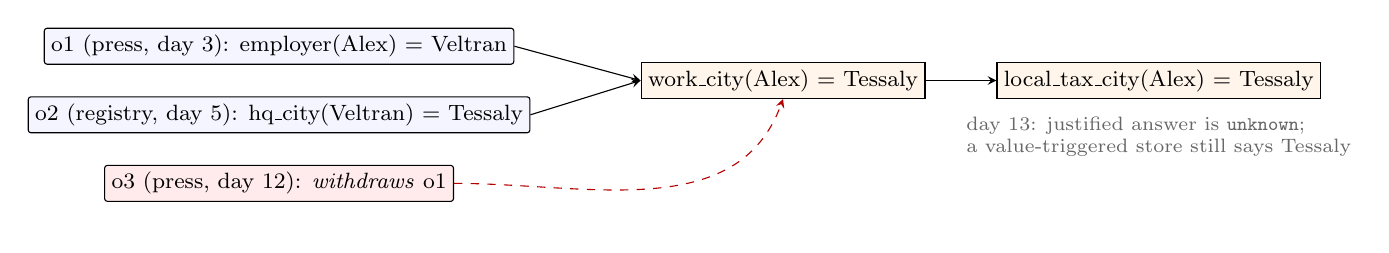
\begin{tikzpicture}[>=stealth, node distance=4mm and 9mm, every node/.style={font=\footnotesize}, obs/.style={draw, rounded corners=1pt, inner sep=2.5pt, fill=blue!4}, der/.style={draw, inner sep=2.5pt, fill=orange!8}, lab/.style={font=\scriptsize, text=black!60}]
\node[obs] (o1) {o1 (press, day 3): employer(Alex) = Veltran};
\node[obs, below=of o1] (o2) {o2 (registry, day 5): hq\_city(Veltran) = Tessaly};
\node[der, right=of $(o1.east)!0.5!(o2.east)$, xshift=6mm] (w) {work\_city(Alex) = Tessaly};
\node[der, right=of w] (t) {local\_tax\_city(Alex) = Tessaly};
\draw[->] (o1.east) -- (w.west); \draw[->] (o2.east) -- (w.west); \draw[->] (w) -- (t);
\node[obs, fill=red!8, below=of o2] (r) {o3 (press, day 12): \emph{withdraws} o1};
\draw[->, red!70!black, dashed] (r.east) to[out=0, in=250] (w.south);
\node[lab, below=1mm of t, align=left] {day 13: justified answer is \texttt{unknown};\\ a value-triggered store still says Tessaly};
\end{tikzpicture}
\caption{A retraction consequence. Derived beliefs are justified by the reports they were derived from (solid arrows). The withdrawal of o1 removes the only justification of both derived beliefs although no report about them changed. Scoring is against what the surviving evidence \emph{justifies}, not against the world.}\label{fig:example}
\end{figure}

Three layers have to be kept apart to study this. The \emph{world} is what is actually the case; it is hidden from every system and used only to generate reports. The \emph{observations} are what sources reported, when, with what reliability class, and which reports were later withdrawn or corrected. \emph{Justified belief} is what the observations warrant under declared assumptions: not the world (a true belief held for no good reason earns nothing), and not the latest report (a later statement is evidence, not truth). Systems are scored against the third layer. Two design commitments follow. The reference reasoner sees only the observations and the declared assumptions, never the world, and when the evidence does not decide between readings it \emph{retains} them rather than selecting one (\S\ref{sec:semantics}). And the requirement to preserve that uncertainty is placed on observable behaviour through a shared output contract (\S\ref{sec:contract}), so that a system representing hypotheses explicitly and an LLM adjudicating a flat log compete on equal terms.

What the study shows. (i)~A declared semantics of justified belief for observation streams with operator cues, dispute, correction and withdrawal, whose per-key implementation is validated against a brute-force global enumeration on \ovQueries{} value queries (Appendix~\ref{app:semantics}), and a benchmark generator, \rs, that separates the three layers with a declared menu of perturbations. (ii)~\pal, an incremental store in which derived beliefs pin the versions of the evidence that justified them, returns the same status, value and alternatives as a symbolic replay of the same semantics on every query of every setting (after one bug fix we report; provenance lists differ on 2--5\%), at six to twelve times lower measured query latency; its total work is lower than replay only when queries are at least as frequent as observations or histories are long, and its write cost grows exponentially in reports per key (\S\ref{sec:res-systems}). (iii)~Within that implementation, retraction propagation through justifications, not ordinary belief updating, is what prevents downstream errors: switching it off costs about 20 points on warranted downstream queries in every setting and nothing on direct ones. (iv)~A regime analysis against the hidden world quantifies what refusing to assume recency buys and costs: last-write-wins is right on about 92\% of value queries whenever the latest report is true (\rgLatestTruePct\% of the queries in our generator) and on 3--12\% when it is delayed or erroneous; justified belief abstains on 20--45\% of the former and on 59--94\% of the latter; a pre-registered same-origin self-update rule removes the abstention in the single-source case at a cost of at most 1.3 points of wrong commitments where the latest report is wrong (\S\ref{sec:res-regime}). (v)~Under automatically extracted assertions with a fixed, declared rule schema, symbolic justification maintenance beats a prompted LLM adjudicator over the same claims by \sTwoHOne{} points on warranted downstream queries while committing on about a seventh as many unresolved slots; a rule-based adjudicator over the same claims scores the same as \pal, so this is a result about the evaluated adjudicators, not about write time versus query time (\S\ref{sec:res-s2}). (vi)~One pre-registered hypothesis fails (calibration) and one could not be executed as registered (the matched-cost clause of H1); the corruption curve locates the error rates at which last-write-wins overtakes justified belief; and when the latest report is an attacker's injection the store commits to it on \rgPoisPalInj{} of queries against \rgPoisLwwInj{} for recency.

Retraction propagation as a \emph{mechanism} is not new: incremental view maintenance keeps derived relations consistent under base-table changes \citep{gupta1993}, justification- and assumption-based truth maintenance withdraw conclusions whose premises are withdrawn \citep{doyle1979,dekleer1986}, MemTX cascades typed repair through derived records in transactional agent memory \citep{memtx2026}, and CUPMem invalidates dependent attributes at write time \citep{stale2026}. Our contribution is the measurement: a semantics and a scoring contract under which premature commitment is visible, a benchmark in which the three layers are separable, and the operating regimes, costs and failure modes of maintaining justifications, including the ones that went against the method.


\section{Related work}
\paragraph{Belief revision and truth maintenance.} AGM revision \citep{agm1985} and belief-base postulates \citep{hansson1999} define rational change of a theory; Katsuno and Mendelzon \citep{km1991} distinguish \emph{update} (the world changed) from \emph{revision} (we were wrong), a distinction our operator cues make observable. Justification- and assumption-based truth maintenance \citep{doyle1979,dekleer1986} maintain which conclusions remain supported when premises are withdrawn; our oracle is an ATMS over environments of accepted reports and \pal{} a JTMS-like store with versioning. Incremental view maintenance \citep{gupta1993} keeps derived relations consistent under base changes; our systems benchmark is that question posed for justifications with alternatives. Non-prioritised revision \citep{hansson1997,makinson1997} allows input to be rejected; our admission is non-prioritised in that reliability never resolves disputes at the oracle level.
\paragraph{Temporal and agent memory.} Bitemporal databases \citep{snodgrass} separate valid from transaction time. Among recent agent-memory systems, MemTX \citep{memtx2026} commits beliefs transactionally and cascades typed repair through derived records; CUPMem \citep{stale2026} invalidates dependent attributes at write time; Kumiho \citep{kumiho2026} maps AGM postulates to versioned property-graph operations; TOKI \citep{toki2026} gives a bitemporal operator algebra for contradiction resolution with audit rows; Zep/Graphiti \citep{graphiti2025} build temporal knowledge graphs. Of these, MemTX and CUPMem propagate invalidation through dependencies; none of the papers we examined scores against justified belief with retained alternatives, measures retraction propagation separately from updating, or reports the compute trade-off against replay. We have not run these systems; Table~\ref{tab:cap} states the comparison at the level of documented capabilities.
\begin{table}[t]\centering\small
\caption{Capabilities as documented in the cited papers (not experimentally compared; we read abstracts, method sections and, for MemTX and Nous, the full text). JM = derived beliefs are repaired when a premise is withdrawn or changed; Alt = unresolved alternatives are retained rather than resolved; Bitemp = valid and belief time distinguished; Withdraw = explicit withdrawal of evidence as an operation; Replay = compared against query-time recomputation. ``yes'' = described in the paper; ``n.r.'' = not reported in the paper (which is not evidence that the system lacks it).}\label{tab:cap}
\begin{tabular}{lccccc}\toprule
System & JM & Alt & Bitemp & Withdraw & Replay \\\midrule
MemTX \citep{memtx2026} & yes (cascading repair) & n.r. & partial & yes & n.r. \\
CUPMem \citep{stale2026} & yes (attribute-level) & n.r. & n.r. & n.r. & n.r. \\
StateMem \citep{statemembench2026} & yes (dependency checks, guided recomputation) & n.r. & n.r. & n.r. & n.r. \\
Kumiho \citep{kumiho2026} & edges (use n.r.) & n.r. & versions & n.r. & n.r. \\
TOKI \citep{toki2026} & n.r. & n.r. & yes & audit rows & n.r. \\
Zep/Graphiti \citep{graphiti2025} & n.r. & n.r. & yes & n.r. & n.r. \\
\pal{} (this paper) & yes & yes & yes & yes & yes \\\bottomrule
\end{tabular}
\end{table}
\paragraph{Benchmarks.} STALE \citep{stale2026}, LongMemEval \citep{longmemeval}, LoCoMo \citep{locomo2024} and StateMemBench \citep{statemembench2026} test memory updates and state tracking against a reference that is the latest or the true state. StateMemBench is the closest in spirit: its benchmark includes stale derived values and a control against excessive updating, and its StateMem method uses deterministic dependency checks with guided recomputation, which is justification maintenance without retained alternatives or evidence withdrawal (Table~\ref{tab:cap}; we have read its method description, not run it); \rs{} differs in scoring against justified belief with hidden world state, delayed and unreliable observations and evidence withdrawal. Knowledge editors have been shown to leave many consequences of an edit unchanged \citep{rippleedits}, a related but distinct failure.
\paragraph{Calibration and source reliability.} Nous \citep{nous2026a,nous2026b} studies reliability-conditioned updating and shows that learning useful state decisions can need far fewer records than calibrating sources; we take from it the choice of decision-relevant metrics (risk--coverage) alongside Brier and ECE, and class-level rather than per-source priors.

\section{Semantics of justified belief}\label{sec:semantics}
We fix a small claim language and define, for any stream of observations, the set of \emph{admissible interpretations} and the beliefs they justify. Everything in this section is a declared benchmark assumption; the oracle never sees the world.

\paragraph{Claim language.} A domain declares entities $E$, attributes, and rules. Each attribute $a$ declares a value type, a cardinality (\texttt{single} or \texttt{multi}), whether it is \texttt{changeable} (volatile vs.\ stable), whether a report of it may be hypothesised erroneous (\texttt{error\_allowed}), and whether differing values on one key are evidence against each other (\texttt{competing\_values}; two residences compete, two nicknames coexist). A proposition is $(e,a,v)$ on key $(e,a)$. Rules are Horn clauses, \texttt{strict} or \texttt{defeasible} with declared exceptions; heads are derived attributes (e.g.\ $\mathit{work\_city}(e)\leftarrow \mathit{employer}(e,x)\wedge \mathit{hq\_city}(x,c)$ unless $\mathit{remote}(e)$).

\paragraph{Time and observations.} Valid time is an integer day; belief time is report time. An \emph{assertion} is $(\mathit{id}, t_{\mathrm{rep}}, \mathit{source}, e,a,v, \mathit{valid\_cue}, \mathit{op\_cue})$ where the valid cue is \texttt{none}, \texttt{since}~$t$ or \texttt{at}~$t$ and the operator cue is \texttt{none}, \texttt{change} (optionally \emph{from} $v_{\mathrm{prev}}$) or \texttt{correction} (\emph{of} a report id). A \emph{retraction} withdraws a report or every report of a source for all later belief times. Sources declare a reliability class (\texttt{trusted}, \texttt{standard}, \texttt{low}, \texttt{blocked}) and an \emph{origin}; sources sharing an origin are copies. A report with no temporal cue is taken to assert that the value held at least at reporting time (A1); \texttt{since}~$t$ anchors it at $t$ and \texttt{at}~$t$ asserts it at $t$. Absent later evidence of a different value, a value persists from its anchor (A4, inertia); the valid cue fixes when a value is known to hold, never when it stops, so inertia applies to \texttt{at} reports exactly as to the others.

\paragraph{Admission and withdrawal.} Policy P0: every report from a non-blocked source is admitted; reliability classes never affect admissibility, only the support layer. A correction whose source shares the origin of the corrected report \emph{withdraws} that report (A-SELF): an origin's later statement about its own earlier statement is a withdrawal, not a competing report. A correction from another origin is a competing report with a cue.

\paragraph{Dispute and contradiction.} Two admitted assertions on the same key are \emph{disputed} iff they have different values and the attribute declares competing values. A \emph{contradiction} between two accepted assertions arises only for single-valued keys when the attribute is stable, or when the attribute is changeable and the two are anchored at the same time. Dispute licenses the hypothesis of error; contradiction forbids joint acceptance. The distinction is what makes ``the London report may be wrong'' admissible even when London-then-Paris is consistent as a change.

\paragraph{Interpretations.} At belief time $\tau$, an interpretation labels every admitted assertion \textsc{true} or \textsc{err}, and every maximal run of accepted same-valued reports on a multi-valued changeable key that is followed by a different value \textsc{cont} or \textsc{ended}. It is admissible iff:
(A-ERR) a report may be \textsc{err} only if error is allowed and some \emph{accepted} competitor disputes it, or an accepted correction targets it---every error label is explained by an accepted competing report, and ``everything is wrong'' is never admissible;
(A-CORR) an accepted correction forces its target \textsc{err};
(A-CHG) an accepted change \emph{from} $v_{\mathrm{prev}}$ presupposes the previous value: if any report of $v_{\mathrm{prev}}$ is anchored strictly earlier, at least one must be accepted (a presupposition about the value, not about a particular report), and on a multi-valued key the run of $v_{\mathrm{prev}}$ preceding the change is labelled \textsc{ended} (the \emph{from} clause states that the previous value stopped);
(A-CUE, policy P0c) a report carrying a change cue is not disputed by competitors anchored strictly earlier than itself---the cue identifies the revision operator, so the earlier value is explained rather than contested---while same-time and later competitors still dispute it;
(A-CONS) no contradiction among accepted reports.
Minimality is deliberately \emph{not} imposed: preferring fewer error labels would make ``London$\to$Paris was a move'' established and ``the London report was wrong'' inadmissible, which is exactly the premature commitment the benchmark is designed to penalise. Preferences belong to the support layer. An interpretation is identified by its \textsc{err} set and the timelines it induces; keys are independent, so interpretation sets are computed per key, and the oracle is made total by a declared relaxation ladder that is counted whenever it fires (it never fires on generated streams under P0c).

\paragraph{Timelines and answers.} Under an interpretation, each accepted run holds from its first anchor; on single-valued keys it ends at an unknown change point in the gap before the next different accepted anchor; on multi-valued keys it persists (\textsc{cont}) or ends in that gap (\textsc{ended}). The value at $t$ inside a gap is $\{v_{\mathrm{prev}}\}$ or $\{v_{\mathrm{next}}\}$---unknown change dates are uncertainty by construction. Derived attributes are forward-chained per interpretation, branching over candidate sets; a defeasible rule whose exception holds contributes nothing.

\paragraph{Gold.} For a value slot, the candidates are the union over interpretations: one candidate $\Rightarrow$ \texttt{established}; several $\Rightarrow$ \texttt{unresolved} with exactly that set; none $\Rightarrow$ \texttt{unknown}. For a multi-valued slot a candidate is a \emph{set} of values and alternatives are sets (London-only, Paris-only and both are three alternatives, never flattened), and the empty set is a candidate like any other: when every interpretation justifies no member---nothing admitted on the key, or everything withdrawn---the slot is \texttt{established} with $\emptyset$, which reads ``no affiliation is justified'' and is distinct from \texttt{unknown} (no interpretation at all, or an undeclared key). A yes/no proposition true in every interpretation is \texttt{established} (false in every one: established with negative polarity---the semantics is closed over the admitted evidence, so a value never asserted does not hold); mixed $\Rightarrow$ \texttt{possible}. These three conventions (empty set, established-false, unknown) are part of the contract and, as \S\ref{sec:res-s3} reports, the one for empty sets was missing from the instruction the LLM adjudicators received. A downstream query asked right after a retraction is a \emph{warranted-retraction consequence} iff its gold is established and differs from its gold one belief step earlier; only such queries enter the primary endpoint.

\paragraph{Worked case.} With \emph{residence} declared multi-valued and competing, after ``Alex lives in London'' (o1) and ``Alex lives in Paris'' (o2) with no cues, exactly four interpretations are admissible: both accepted with London continuing (both residences), both accepted with London ended (a move), o1 in error, o2 in error. ``Did Alex move?'' is \texttt{possible}; ``Was the London report wrong?'' is \texttt{possible}; ``Which residences were reported?'' is \texttt{established} with provenance; ``Which city's tax applies?'' (a rule on residence) is \texttt{unresolved} over three alternatives and is not a warranted consequence. Had o2 said ``Alex moved from London to Paris'', the move would be established under A-CUE. Two independent implementations of this semantics (a constructive per-key enumeration and a brute-force global one) were compared on the three hand-written reference streams, where they agree on the interpretation sets and the gold of every query at every belief time; on the 500 generated streams only the weaker check that every key has at least one admissible interpretation under P0c was run (the global oracle does not scale to them). The incremental store and the symbolic replay, which share the per-key oracle, are compared on every query of every setting in \S\ref{sec:res-systems}.

\paragraph{Self-update (A-SU, variant P0cSU).} A later uncued report from the \emph{same origin} on a single-valued changeable key is, under P0c, a dispute with the origin's own earlier report. The regime analysis of \S\ref{sec:res-regime} and an external check showed this to be a poor default for self-report streams. The Bayesian argument depends on the observation model, and we state both that we considered. Let two reports of one source on one key differ in value; let $c$ be the probability that the world value changed between them and $e$ the probability that a report is erroneous, independently. Under a \emph{binary} value model (an erroneous report shows the only other value), $P(\text{later value is current}\mid\text{values differ})=\frac{c(1-e)^2+(1-c)e(1-e)}{c[(1-e)^2+e^2]+2(1-c)e(1-e)}$, which exceeds $\tfrac12$ by $c(1-2e)/(2\cdot\text{denominator})$, i.e.\ for every $c>0$ and $e<\tfrac12$ (an earlier draft omitted the $ce^2$ term, which inflated the value at large $c$). Under an \emph{open} value model (an erroneous report shows a value distinct from both the true ones), the same probability is $\frac{c(1-e)+(1-c)e(1-e)}{c+(1-c)(2e-e^2)}$, which exceeds $\tfrac12$ only when $c(1-2e)\ge(1-c)e(1-e)$, roughly when changes are at least as likely as errors. In either model the later value is the better \emph{guess} in the stated regime; a probability above one half supports a preference, not a justification, so A-SU is a declared policy choice and not a theorem. A-SU, pre-registered before it was implemented (Appendix~\ref{app:chronology}), forbids labelling a report \textsc{err} when every accepted competitor is a strictly-earlier report from its own origin and no correction targets it; it never defeats a later competitor, a correction or a withdrawal, and does not apply to stable attributes. It is adopted as the default for self-report streams and reported as the declared variant P0cSU elsewhere; its measured cost is in \S\ref{sec:res-regime}; the frozen results of Settings 1--3 are under P0c.

\paragraph{Variants.} Literal P0 (no cue shields any report: only withdrawal resolves) and P1 (class-prioritised dispute: a lower-class report disputes a higher-class one only when corroborated from a second origin) are implemented and reported as sensitivity analyses. P1 is not the main configuration because it builds a reliability ordering into the oracle that the systems under test are meant to estimate, and because it marks a trusted source's false statement \texttt{established} whenever only lower-ranked sources contradict it.


\section{The output contract}\label{sec:contract}
The requirement to preserve uncertainty is placed on \emph{observable behaviour}, not on internal representation: the scoring must not favour a system that stores hypotheses over one that reasons at query time. Every system, including the references, answers through one JSON object: a \texttt{status} in \{\texttt{established}, \texttt{possible}, \texttt{unresolved}, \texttt{unknown}\}, an \texttt{assertion}, an \texttt{alternatives} list, and \texttt{provenance} (observation ids); an optional free-text explanation is never scored. The statuses are defined operationally and are mutually exclusive: \texttt{established} means supported under every admissible interpretation given the declared assumptions, never independently verified truth; \texttt{possible} qualifies one proposition that holds under some interpretations; \texttt{unresolved} declines to choose between candidate values and must list them; \texttt{unknown} has no candidates. The shared instruction contains these definitions and the Alex examples verbatim and is identical for every system, as is the vocabulary (entity ids, attribute types and normalisation, observation ids). Nothing exposes gold labels or hidden dependency rules beyond what the setting declares.

\paragraph{Deterministic scoring.} Values are canonical (entity ids, ISO dates, lower-cased strings; sorted lists for multi-valued slots), so credit is exact: status must match, and the assertion or the alternative set must equal the gold after normalisation. Selecting one interpretation on an \texttt{unresolved} or \texttt{possible} slot scores zero on that query and counts as a \emph{premature commitment}. A lenient variant (superset of alternatives) was defined but is not reported in this version; all numbers are exact-match. No LLM judge is used in Settings 1--2.

\paragraph{Provenance.} A cited observation id is \emph{supporting} when it asserts a (key, value) binding that lies on an oracle justification path for the answer: for a derived slot the rule engine records the bindings used along every derivation that yields a candidate value. Provenance precision and recall are secondary metrics; an existing but non-supporting id earns nothing.

\paragraph{Malformed outputs.} Outputs are validated against the schema and vocabulary; exactly one repair attempt with a fixed, system-independent prompt is allowed and charged to the system; a second failure is scored wrong on every query (never as abstention) and the malformed rate is reported (it is zero for every system in every run; the repair was invoked once in the Haiku runs and on 192 of 994 answers in the Sonnet subset).

\paragraph{References.} Always-abstain answers every value slot \texttt{unresolved} over the reported values (and yes/no slots \texttt{possible}); always-commit takes the most recent report at face value. Neither is a competitor: a real system must beat always-abstain on resolvable queries and always-commit on unresolved ones, otherwise uncertainty handling has become an escape from answering, or commitment an escape from reasoning.


\section{\rs{} and the evaluation settings}\label{sec:benchmark}
\rs{} separates three layers per stream: the world trajectory (hidden from every system, used only for calibration and for the attacker), the observation stream with provenance (what systems see), and the oracle's justified beliefs (gold, computed from the observations alone).

\paragraph{World and reporting.} A seeded simulator draws persons, organisations and cities with attributes \emph{employer, residence (multi-valued), remote, birth\_date, nickname (non-competing), hq\_city, ceo}, three rules (\emph{work\_city, local\_tax\_city, ceo\_city}; one chained, one with a defeasible exception), and changes of volatile attributes over a 60-day horizon with occasional reversals. Eight sources in four classes report each world fact one to three times with geometric delays and a heavy tail (10--25 days), with an explicit \texttt{since} cue half the time on changeable attributes, with change cues on a third of change reports (half of them with a stated previous value), and with class-specific error rates (trusted 6\%, standard 12\%, low 30\%). Two sources are copies of others (same origin). An erroneous report is followed with declared probabilities by a self-correction (A-SELF), by a cross-origin correction from a random source that is low-trust half the time (a genuine low-trust correction), or by nothing. Reports are explicitly retracted at a rate that favours erroneous ones, and one non-trusted source is retracted wholesale in a third of streams. Per-key report counts are capped at seven to bound enumeration. The attacker model (secondary RQ) injects false assertions at a declared rate through a fresh low-trust channel or a compromised trusted channel, half of them with a false change cue.

\paragraph{Queries.} Event-driven queries are asked at every retraction, correction and cued change: the affected key (\texttt{current}), every derived key whose justification can depend on it (\texttt{downstream}, found by inverting the oracle's own dependency relation), the relevant yes/no propositions (\emph{erroneous}, \emph{changed}), each with a companion asked one belief step earlier. Grid queries sample the bitemporal cells: as-of valid time, as-of belief time (``what was justified on day $\tau'$''), \emph{holds}, and \texttt{reported}. The declared selection keeps at most 44 primary queries per stream (a cap, not a guaranteed count: a stratum shorter than its quota is not padded): 35\% warranted-retraction consequences (downstream first), 25\% non-warranted event queries (they feed the instability endpoint), 40\% grid queries balanced between resolvable and unresolved, plus the $\tau-1$ companions of event queries and the \texttt{reported} slots, which are scored separately. Generated streams average 131 observations and about 280 candidate queries before selection; the frozen Setting 1 set has 60.5 queries per stream (37.1 primary, 20.5 companions, 2.9 \texttt{reported}; 30{,}272 in all), of which \sOneWarrPerStream{} per stream are warranted downstream queries; the frozen Setting 2 set has 67.4 per stream (40.6 primary, 23.4 companions, 3.4 \texttt{reported}; 6{,}737 in all) and \sTwoWarrPerStream{} warranted downstream queries per stream (741 in total).

\paragraph{Natural-language setting.} Each observation is rendered as a report line ``[id] (outlet, date): sentence'' by templates with fictional names (so no world knowledge can be leaned on), paraphrased by a cheap model, and passed through a cue-recovery check---deterministic markers plus a cheap-model pass blind to the structured source---with up to two regenerations; lines that still fail are adjudicated by stripping the lost cue from the \emph{frozen label}, so gold reflects the text as presented. The evaluation set is then frozen. A shared extractor turns every line into a structured claim under the declared attribute and rule schema (the rules are given, not extracted); its slot errors, \emph{missed ambiguity} (text has no cue, extractor added one) and \emph{spurious ambiguity} (text has a cue, extractor dropped it) are measured against the frozen labels, and an extractor's declaration never changes which queries are answerable.


\section{Systems}\label{sec:systems}
\paragraph{\pal.} A write-time belief store. Every observed key holds an append-only list of versions (belief time, admitted report ids, interpretation set computed with the declared semantics); every derived belief (entity, derived attribute) holds versions that \emph{pin} the key versions it was justified by. Answers at belief time $\tau$ are read from the versions in force at $\tau$, so bitemporal questions are lookups. On an assertion, the key is recomputed and every dependent derived belief is refreshed (ordinary belief updating). On a retraction or withdrawal, the key is recomputed and---this is the propagation step---every derived belief that depends on it is refreshed. Support (\S\ref{sec:support}) is computed from the admitted evidence of a key. In the natural-language setting the store reasons over the shared extracted claims; the LLM is used only at the boundary (extraction), never to answer.

\paragraph{Ablations.} \emph{No propagation}: a retraction updates the retracted key only; derived beliefs keep their pinned versions until an ordinary assertion refreshes them. \emph{Forced commit}: each key keeps a single interpretation, the admissible one with fewest error labels (ties: ended over continuing). Further ablations of the support model are reported with RQ3.

\paragraph{Symbolic replay (the equivalence baseline).} The same claims in an append-only log; at query time the semantics is executed from scratch over the log filtered to the query's belief time: every key the query depends on is re-enumerated and the derived value re-chained, with the per-key cache cleared before each query (\emph{cold}) or retained across queries (\emph{cached}): the cache is a memo keyed by (key, belief time, policy) that is never invalidated, which is sound because the log is append-only and a report at a later belief time cannot change an earlier belief time's interpretation set; it therefore helps only when a later query touches the same key at the same belief time. Replay and \pal{} execute the same declared semantics on the same evidence and have no information the other lacks; they must agree on every answer, and \S\ref{sec:res-systems} verifies that they do and measures what each costs. In the natural-language settings replay is the ``log + rule adjudicator'' row: what query-time reasoning achieves over the extracted claims when the reasoning is correct.

\paragraph{Append-only log with LLM adjudication.} The same extracted claims in the same log; at query time the backbone LLM receives the log filtered to the query's belief time, the declared attribute and rule block, the shared instruction, and the query rendered as its answer slot, and must return the contract JSON, with one repair attempt. Context-budget variants restrict the log to the $k$ most recent entries plus every entry on the queried key ($k\in\{10,20,40\}$); a raw-report variant adjudicates the natural-language reports directly, with no extraction. Relative to \pal{} this comparison changes two things at once, who reasons (a prompted model instead of a rule engine) and when (query time instead of write time); replay, which reasons with the rule engine at query time, separates them.

\paragraph{Temporal DB (last write wins).} A rule-based bitemporal store without justifications: the record with the latest valid-time anchor wins, retractions remove records, no error hypotheses, derived values computed at query time. It differs from \pal{} in two respects at once, no justifications and a commit-always uncertainty policy, so its gap is not attributed to one of them; the always-commit reference (latest report by report time) isolates pure recency.

\paragraph{Support model.}\label{sec:support} Support is the probability that a candidate value is true for its interval, defined from admitted evidence only: evidence is grouped by origin (copies count once), each origin contributes a per-class log-odds (declared, or learned from verified outcomes of training streams), discounted by staleness on changeable attributes with a 20-day half-life, boosted by a change cue, and capped for a report targeted by a correction at half the correcting origin's weight (the min(provenance, content) cap); support of $v$ is the logistic of the net evidence for $v$ against all competitors, with a prior offset when no competitor exists. Source identities are never used, only classes and origins. Support is produced for exactly the alternatives the justified-belief layer keeps open, so the two layers are evaluated separately.


\section{Protocol and pre-registration}\label{sec:protocol}
\paragraph{Endpoints.} The primary endpoint is exact-match accuracy on warranted-retraction consequence queries on \emph{downstream} slots (propagation through justifications); the same on the retracted key itself is secondary (ordinary updating). Ambiguity is measured separately and never pooled with the primary: the premature-commitment rate on unresolved/possible slots, and the answer-instability rate (registered as ``unsupported propagation'': share of non-warranted event queries whose answer changed between the companion and the event while the gold did not), decomposed post hoc into correct/wrong transitions because the registered form counts beneficial changes as failures, reported next to resolvable accuracy and the two references so that abstention cannot buy a low commitment rate. Calibration is claim-level Brier, ECE (15 equal-mass bins) and the area under the risk--coverage curve. Cost is input plus $8\times$ output tokens (the backbone's price ratio) summed over ingestion, repair and answering, with contract tokens charged at full price. The stream is the unit of analysis: paired per-stream differences with a 10{,}000-resample cluster bootstrap and effect sizes with 95\% intervals.

\paragraph{Pre-registered hypotheses.} H1 (primary): in Setting 2 on warranted downstream queries, \pal{} exceeds the LLM-adjudicated log at matched cost by $\geq 10$ points with an interval excluding zero; falsified if the interval includes zero under extracted dependencies, unfamiliar sources and matched cost together, in which case the cost-crossover analysis is the main finding. H2: a crossover query-to-update ratio $r^*<1$ exists. H3: the evidence model's support has lower ECE than verbalised confidence on held-out sources. H4 (joint): lower premature-commitment rate than the log baseline \emph{and} resolvable accuracy not lower by more than 3 points. H2--H4 use Holm correction (\S\ref{sec:threats} reports why it changes no conclusion). H1's ``matched cost'' clause could not be executed as registered; \S\ref{sec:res-s2} reports the context-budget curve that replaces it. Appendix~\ref{app:chronology} gives the dated chronology of every decision, including those taken after results were seen. Phase gates preceded any paid run: two independent oracles must agree; a propagation-off store must score measurably worse on warranted downstream queries; the references must split; a forced-commit store must raise unsupported propagation. The pre-registration, with every deviation dated, is released with the code.

\paragraph{Deviations recorded.} (i) The planned backbone (GPT-5 mini via a batch API) and Amazon Bedrock were unreachable from the execution environment; Claude Haiku 4.5 through the Anthropic Message Batches API (50\% discount, prompt caching on the shared instruction) was used for every stage, and Claude Sonnet 4.6 on 15 streams as the sign-stability check. (i$'$) Setting 2 ran on 100 streams rather than 150 to keep total spend under the \$100 ceiling (interval half-width 0.04 at the observed spread); the raw-report log and the matched-cost variant ran on 30 streams. Total measured spend for every LLM call in the study, including development, two discarded batches and the post-review reruns, was \$\spendTotal. (ii) The warranted-query floor of 8 per stream was met on development streams by raising the primary query budget from 40 to 44 with quota 35/25/40 before the freeze; the frozen Setting 1 set has \sOneWarrPerStream{} and the frozen Setting 2 set \sTwoWarrPerStream{} (741 queries; 99 of 100 streams contribute to the primary estimate); generator rates were not changed. (iii) Query counts (\S\ref{sec:benchmark} gives the per-stream flow): the \sOneAnswers{} ``scored answers'' of Setting 1 are the primary queries whose gold is \texttt{established}, \texttt{unresolved} or \texttt{possible} (companions, \texttt{reported} slots and \texttt{unknown}-gold queries excluded); the Setting 2 totals are 6{,}737 queries, 4{,}062 primary, 741 warranted downstream; the literal-P0 yield of 2.3 warranted downstream queries per stream was measured on development streams before the selection rule, the 3.38 of the sensitivity table after it. (iv) The dispute semantics changed from literal P0 to P0c after Phase 1 measurement (literal P0 leaves 2.3 warranted downstream queries per stream and 48\% unresolved slots), with literal P0 retained as a sensitivity variant; and the change presupposition (A-CHG) was weakened from a specific report to the value after it produced inconsistent streams.


\section{Results}\label{sec:results}
\subsection{Semantic agreement and the cost of maintaining justifications}\label{sec:res-systems}
\begin{sidewaystable}\centering\small
\caption{Incremental justification maintenance vs symbolic replay of the same semantics on the same streams and queries (no LLM). CPU seconds per stream (process time), query latency mean / p95 / max in ms, peak traced memory in MB; $r$ = queries per observation. Answers agree on every query (last column: disagreements / answers). Scale rows: generated streams with $m$ reports per key and horizon $T$ days, $r=1$.}\label{tab:sys}
\begin{tabular}{llrrrrrrrr}
\toprule
Workload & System & CPU total & CPU write & lat.\ mean & p95 & max & mem & recomputes & disagree \\
\midrule
Setting 1, r=0.1 & incremental & 0.33 & 0.32 & 0.4 & 1.0 & 12 & 1.0 & 136 & 0/799 \\
 & replay cold & 0.03 & 0.00 & 2.6 & 6.7 & 61 & 0.1 & 17 &  \\
 & replay lazy & 0.04 & 0.00 & 2.6 & 6.8 & 98 & 0.2 & 17 &  \\
\addlinespace[2pt]
Setting 1, r=0.33 & incremental & 0.32 & 0.31 & 0.4 & 1.2 & 10 & 0.9 & 136 & 0/2637 \\
 & replay cold & 0.11 & 0.00 & 2.6 & 9.2 & 69 & 0.3 & 57 &  \\
 & replay lazy & 0.11 & 0.00 & 2.5 & 9.4 & 73 & 0.5 & 56 &  \\
\addlinespace[2pt]
Setting 1, r=1.0 & incremental & 0.36 & 0.32 & 0.4 & 1.5 & 57 & 1.0 & 136 & 0/7974 \\
 & replay cold & 0.32 & 0.00 & 2.4 & 11.0 & 79 & 0.5 & 173 &  \\
 & replay lazy & 0.32 & 0.00 & 2.4 & 11.1 & 117 & 1.3 & 165 &  \\
\addlinespace[2pt]
Setting 1, r=3.0 & incremental & 0.46 & 0.32 & 0.3 & 1.6 & 40 & 1.2 & 136 & 0/23922 \\
 & replay cold & 0.93 & 0.00 & 2.3 & 11.7 & 85 & 0.7 & 520 &  \\
 & replay lazy & 0.87 & 0.00 & 2.2 & 11.1 & 81 & 3.2 & 449 &  \\
\addlinespace[2pt]
scale $m$=10, $T$=120, $r$=1.0 & incremental & 2.15 & 1.89 & 1.3 & 7.0 & 56 & 8.5 & 206 & 0/992 \\
 & replay cold & 3.16 & 0.00 & 15.7 & 91.2 & 487 & 1.8 & 248 &  \\
 & replay lazy & 3.09 & 0.00 & 15.4 & 82.5 & 481 & 11.0 & 240 &  \\
\addlinespace[2pt]
scale $m$=10, $T$=60, $r$=1.0 & incremental & 0.97 & 0.86 & 0.8 & 1.9 & 57 & 4.1 & 134 & 0/668 \\
 & replay cold & 1.10 & 0.00 & 8.3 & 31.5 & 597 & 1.5 & 176 &  \\
 & replay lazy & 1.01 & 0.00 & 7.7 & 29.7 & 597 & 3.9 & 167 &  \\
\addlinespace[2pt]
scale $m$=13, $T$=60, $r$=1.0 & incremental & 3.72 & 3.61 & 0.9 & 1.8 & 215 & 22.4 & 138 & 0/686 \\
 & replay cold & 1.66 & 0.00 & 12.5 & 34.3 & 2553 & 4.2 & 183 &  \\
 & replay lazy & 1.62 & 0.00 & 12.2 & 32.2 & 2475 & 7.2 & 174 &  \\
\addlinespace[2pt]
scale $m$=7, $T$=120, $r$=1.0 & incremental & 0.57 & 0.48 & 0.6 & 2.7 & 11 & 1.9 & 166 & 0/800 \\
 & replay cold & 0.66 & 0.00 & 4.2 & 19.6 & 73 & 0.7 & 227 &  \\
 & replay lazy & 0.68 & 0.00 & 4.4 & 18.0 & 104 & 2.7 & 218 &  \\
\addlinespace[2pt]
scale $m$=7, $T$=240, $r$=1.0 & incremental & 0.79 & 0.61 & 0.9 & 4.1 & 16 & 2.9 & 187 & 0/934 \\
 & replay cold & 1.38 & 0.00 & 7.4 & 31.7 & 108 & 1.1 & 259 &  \\
 & replay lazy & 1.42 & 0.00 & 7.6 & 31.3 & 177 & 5.3 & 254 &  \\
\addlinespace[2pt]
scale $m$=7, $T$=60, $r$=1.0 & incremental & 0.34 & 0.30 & 0.3 & 1.4 & 11 & 1.1 & 129 & 0/618 \\
 & replay cold & 0.24 & 0.00 & 2.0 & 8.2 & 45 & 0.4 & 161 &  \\
 & replay lazy & 0.24 & 0.00 & 2.0 & 8.3 & 49 & 1.0 & 153 &  \\
\addlinespace[2pt]
\bottomrule
\end{tabular}
\end{sidewaystable}
\begin{figure}[t]\centering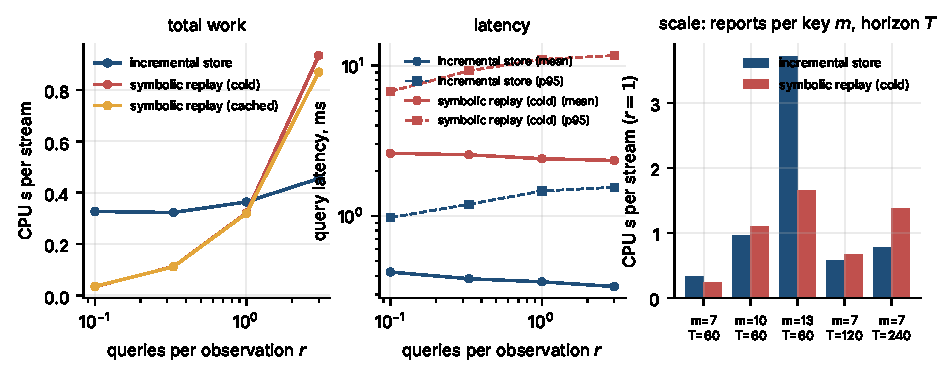
\includegraphics[width=\textwidth]{figures/systems.pdf}
\caption{Incremental maintenance vs symbolic replay on the same streams and queries (no LLM). Left: CPU per stream against the query/observation ratio; replay is cheaper below $r\approx1$, maintenance above. Centre: query latency (mean and p95). Right: total CPU at $r=1$ as reports per key $m$ and horizon $T$ grow; the store's per-write enumeration dominates at $m=13$.}\label{fig:systems}
\end{figure}
The first result is an equivalence, stated by field. \pal{} and symbolic replay execute the same semantics on the same evidence and must return the same status, assertion and alternatives; on every query of every setting they now do: the 30{,}272 queries of Setting 1 (both equal the oracle), the 6{,}737 of Setting 2, the 714 of Setting 3, the 994 of the Sonnet subset, and the \sysAnswers{} queries of the workload study in Table~\ref{tab:sys}, with \sysDisagree{} disagreements on those three fields. The provenance lists differ on 2.3\% of Setting 2 and 5.3\% of Setting 3 queries, the store citing the observations of the pinned key versions and replay the observations on justification paths, which is why their provenance precision differs by about a point; the full contract JSON is therefore not identical, the scored fields are. They did not at first: 18 of 6{,}737 Setting 2 answers differed, all of one kind---an extracted correction whose entity and value the extractor had swapped landed on a different key from its target, replay applied the same-origin withdrawal (A-SELF) globally and the store applied it only on the correction's own key. The fix is recorded as a dated deviation; the structured systems were re-scored from the cached extractions, which moved \pal's Setting 2 warranted downstream accuracy from 0.953 to \sTwoPalWarr, direct accuracy from 0.993 to 0.996, resolvable accuracy from 0.975 to 0.976 and commitment from 0.082 to 0.080, and left the LLM rows untouched. We mention it because the reviewer-visible discrepancy of three tenths of a point was a real bug, and because it shows what the equivalence check is for.

The second result is the cost, which the subtitle of an earlier draft asked about and which Table~\ref{tab:sys} and Figure~\ref{fig:systems} answer. At the generator's default scale (133 observations per stream, at most seven reports per key) replay does \emph{less} total work than maintenance when queries are rarer than observations ($r=0.1$: \sysRpOneRepCpu{} vs \sysRpOneIncCpu{}~s per stream; $r=1$: \sysROneRepCpu{} vs \sysROneIncCpu{}), and more when they are more frequent ($r=3$: \sysRThreeRepCpu{} vs \sysRThreeIncCpu{}); the crossing is workload-dependent: interpolating the two measured points around it at default scale puts it near 1.1 queries per observation, with no repeated runs to attach an uncertainty to. Longer histories move it in maintenance's favour (240-day horizon at $r=1$: \sysTTwoFortyRepCpu{} vs \sysTTwoFortyIncCpu{}), more reports per key move it against: at 13 reports per key the per-write enumeration of interpretations costs \sysMThirteenIncCpu{}~s against \sysMThirteenRepCpu{} for replay and \sysMThirteenIncMem{}~MB of peak memory against \sysMThirteenRepMem{}, because the store re-enumerates a key's $2^n$ labelings on every write while replay enumerates only the keys a query touches. What maintenance buys at every scale is measured latency: \sysROneIncLat{}~ms per query against \sysROneRepLat{} at $r=1$, p95 \sysROneIncPNN{} against \sysROneRepPNN{}, and a worst case of \sysMThirteenIncMax{}~ms against \sysMThirteenRepMax{}~ms at 13 reports per key. The summary is that write-time justification maintenance gives the same answers with lower measured query latency, saves total work only when queries are at least as frequent as observations or histories are long, and has a write cost exponential in reports per key that bounds its use without a smarter per-key representation. None of this involves an LLM; it is the systems question separated from the adjudication question. Method: one process on a 2-vCPU Intel Xeon 2.80\,GHz container (Python 3.13, Linux), CPU time by \texttt{time.process\_time}, each (stream, ratio) cell run once in the order incremental, cold replay, cached replay on a fresh copy of the stream, default garbage collection, memory as \texttt{tracemalloc} peak traced allocation (not resident memory); 60 Setting 1 streams per ratio and 5 generated streams per scale cell; latency distributions are over queries, the maxima are single observations, and no interval is attached to the CPU totals.

\subsection{Setting 1: structured streams, gold dependencies}\label{sec:res-s1}
\begin{sidewaystable}\centering\footnotesize\setlength{\tabcolsep}{3.5pt}
\caption{Setting 1 (structured streams, gold dependencies, no LLM; 500 streams). Stream-level means with 95\% cluster-bootstrap intervals.}\label{tab:s1}
\begin{tabular}{lcccccccc}
\toprule
System & Warr.\ downstream & Warr.\ direct & Resolvable & Unresolved & Commit rate$\downarrow$ & Unsupp.\ prop.$\downarrow$ & Prov.\ P & Prov.\ R \\
\midrule
\textsc{Palimpsest} & 1.000 {\tiny[1.00,1.00]} & 1.000 {\tiny[1.00,1.00]} & 1.000 {\tiny[1.00,1.00]} & 1.000 {\tiny[1.00,1.00]} & 0.000 {\tiny[0.00,0.00]} & 0.000 {\tiny[0.00,0.00]} & 0.990 {\tiny[0.99,0.99]} & 0.993 {\tiny[0.99,0.99]} \\
\quad no propagation & 0.794 {\tiny[0.78,0.81]} & 1.000 {\tiny[1.00,1.00]} & 0.933 {\tiny[0.93,0.94]} & 0.962 {\tiny[0.96,0.97]} & 0.002 {\tiny[0.00,0.00]} & 0.017 {\tiny[0.01,0.02]} & 0.981 {\tiny[0.98,0.98]} & 0.989 {\tiny[0.99,0.99]} \\
\quad forced commit & 1.000 {\tiny[1.00,1.00]} & 1.000 {\tiny[1.00,1.00]} & 1.000 {\tiny[1.00,1.00]} & 0.042 {\tiny[0.04,0.05]} & 0.776 {\tiny[0.76,0.79]} & 0.090 {\tiny[0.08,0.10]} & 0.992 {\tiny[0.99,0.99]} & 0.775 {\tiny[0.77,0.78]} \\
Log + rule adjudicator & 1.000 {\tiny[1.00,1.00]} & 1.000 {\tiny[1.00,1.00]} & 1.000 {\tiny[1.00,1.00]} & 1.000 {\tiny[1.00,1.00]} & 0.000 {\tiny[0.00,0.00]} & 0.000 {\tiny[0.00,0.00]} & 1.000 {\tiny[1.00,1.00]} & 1.000 {\tiny[1.00,1.00]} \\
Temporal DB & 0.807 {\tiny[0.79,0.82]} & 0.909 {\tiny[0.89,0.92]} & 0.907 {\tiny[0.90,0.91]} & 0.000 {\tiny[0.00,0.00]} & 0.848 {\tiny[0.84,0.86]} & 0.105 {\tiny[0.09,0.12]} & 0.950 {\tiny[0.95,0.95]} & 0.341 {\tiny[0.33,0.35]} \\
Always abstain & 0.000 {\tiny[0.00,0.00]} & 0.000 {\tiny[0.00,0.00]} & 0.000 {\tiny[0.00,0.00]} & 0.393 {\tiny[0.38,0.41]} & 0.000 {\tiny[0.00,0.00]} & 0.075 {\tiny[0.06,0.09]} & 0.507 {\tiny[0.50,0.51]} & 0.739 {\tiny[0.73,0.75]} \\
Always commit & 0.438 {\tiny[0.42,0.46]} & 0.970 {\tiny[0.96,0.98]} & 0.770 {\tiny[0.76,0.78]} & 0.000 {\tiny[0.00,0.00]} & 0.793 {\tiny[0.78,0.81]} & 0.157 {\tiny[0.14,0.17]} & 0.939 {\tiny[0.93,0.94]} & 0.284 {\tiny[0.28,0.29]} \\
\bottomrule
\end{tabular}
\end{sidewaystable}
Table~\ref{tab:s1} reports all systems on 500 streams (\sOneAnswers{} scored answers per system; Appendix~\ref{app:tables} gives the per-slot breakdown and the dispute-policy sensitivity). \pal{} and replay reproduce the oracle on every query. Removing retraction propagation costs $\sOnePropEffect$ points $[\sOnePropLo, \sOnePropHi]$ on warranted downstream queries (paired over \sOnePropN{} streams) and nothing on direct ones: ordinary belief updating handles the retracted key, only propagation handles its consequences. The forced-commit variant keeps perfect resolvable accuracy while committing on \sOneCommitRate\% of unresolved slots and changing downstream answers after non-warranted events $\sOneCommitUnsup$ points $[\sOneCommitUnsupLo, \sOneCommitUnsupHi]$ more often. The references split as required (always-abstain: \sOneAbstainRes{} resolvable / \sOneAbstainUnres{} unresolved; always-commit: \sOneCommitRes{} / \sOneCommitUnres{}); always-commit scores below one on unresolved slots because yes/no \emph{erroneous} questions and \texttt{reported} slots are answered by rule, not by recency. The temporal DB loses \sOneTdbWarr{} points on warranted downstream queries and commits on \sOneTdbCommit\% of unresolved slots. These are validation results on a benchmark whose generator and system share an author: they establish that the instruments discriminate, not that any hypothesis holds.

\subsection{When is recency right?}\label{sec:res-regime}
\begin{sidewaystable}\centering\small
\caption{When is recency right? Value queries on single-valued keys of 200 fresh generated streams (seeds 20000--20199), classified from the hidden generator labels by what the latest report on the key is; the same queries are scored under P0c and under the self-update variant P0cSU (paired). Accuracy against the hidden world value; LWW = last-write-wins by report time; valid = by valid-time anchor (temporal DB); abst.\ = abstention rate; wrong commit = committed to a value other than the world's (not a transition); argmax = support-ranked commitment on unresolved slots (P0c). $^\dagger$Poisoning row from 60 attack streams (rate 0.2, low channel), P0c only; its last column is the share of queries committed to the injected value (LWW: 1.00). Setting 1 (500 streams) gives the same picture (Appendix~\ref{app:tables}).}\label{tab:regime}
\begin{tabular}{lrcccccccccc}
\toprule
Regime (latest report) & $n$ & LWW & valid & P0c world & P0c abst. & P0c wrong commit & P0cSU world & P0cSU abst. & P0cSU wrong commit & argmax & injected \\
\midrule
self-update (same origin, latest true) & 53 & 0.96 & 0.96 & 0.68 & 0.32 & 0.00 & 0.96 & 0.00 & 0.04 & 0.94 & -- \\
multi-source update (latest true) & 854 & 0.92 & 0.92 & 0.71 & 0.24 & 0.04 & 0.73 & 0.23 & 0.05 & 0.85 & -- \\
earlier report erroneous, latest true & 1427 & 0.92 & 0.90 & 0.56 & 0.41 & 0.04 & 0.57 & 0.39 & 0.04 & 0.84 & -- \\
delayed report (latest true but older) & 75 & 0.12 & 0.32 & 0.11 & 0.63 & 0.27 & 0.13 & 0.59 & 0.28 & 0.35 & -- \\
latest erroneous, low-trust source & 192 & 0.03 & 0.09 & 0.01 & 0.95 & 0.04 & 0.01 & 0.94 & 0.05 & 0.69 & -- \\
latest erroneous, other source & 96 & 0.05 & 0.20 & 0.01 & 0.91 & 0.08 & 0.02 & 0.90 & 0.08 & 0.39 & -- \\
latest report withdrawn & 242 & 0.51 & 0.52 & 0.35 & 0.31 & 0.34 & 0.35 & 0.29 & 0.35 & 0.47 & -- \\
no conflict & 850 & 0.61 & 0.61 & 0.61 & 0.11 & 0.28 & 0.61 & 0.11 & 0.28 & 0.61 & -- \\
latest report is an injection$^\dagger$ & 78 & 0.05 & 0.05 & 0.03 & 0.22 & 0.76 & -- & -- & -- & 0.20 & 0.78 \\
\bottomrule
\end{tabular}
\end{sidewaystable}
\begin{figure}[t]\centering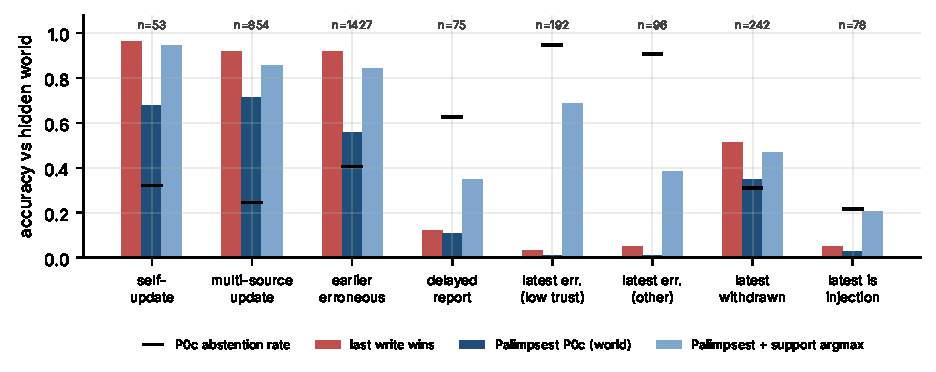
\includegraphics[width=\textwidth]{figures/regime.pdf}
\caption{Accuracy against the hidden world by regime (what the latest report on the key is), value queries on single-valued keys of the 200 fresh streams; poisoning from 60 attack streams. Bars: last-write-wins, \pal{} under P0c, and \pal{} with support-ranked commitment on unresolved slots; ticks: P0c abstention rate.}\label{fig:regime}
\end{figure}
Justified belief is scored against the evidence, but the world is what a user cares about, and the generator knows it. Table~\ref{tab:regime} classifies every value query on a single-valued key of 200 fresh streams by what the latest report on that key is, using the hidden labels, and scores each system against the hidden world value, with P0c and the self-update variant P0cSU on the same queries (the 500 frozen Setting 1 streams give the same picture, Appendix~\ref{app:tables}, Table~\ref{tab:regime-s1}). The pattern is simple. Where the latest report is true---the same origin updating itself (self-update, \rgSelfN{} queries), several origins reporting a change (\rgMultiN), or an earlier report being the erroneous one (\rgStaleN)---last-write-wins is right on \rgSelfLww, \rgMultiLww{} and \rgStaleLww{} of queries and P0c abstains on \rgSelfAbst, \rgMultiAbst{} and \rgStaleAbst{} of them, committing to a non-world value on at most \rgMultiWrong. Where the latest report is wrong---it reports an older fact late (\rgDelayN), or is erroneous from a low-trust (\rgLowN) or another (\rgOthN) source---recency is right on \rgDelayLww, \rgLowLww{} and \rgOthLww, P0c abstains on \rgDelayAbst, \rgLowAbst{} and \rgOthAbst{} and commits to a non-world value on \rgDelayWrong, \rgLowWrong{} and \rgOthWrong. After a withdrawal of the latest report (\rgRetrN) both are near chance against the world because the generator withdraws true reports too: the justified value and the world value come apart by construction. The three ``latest true'' regimes hold \rgLatestTruePct\% of the queries in our generator and the three ``latest wrong'' regimes \rgLatestWrongPct\%; the semantics' refusal to assume recency is paid in the former and earns its keep in the latter.

The poisoning regime is reported as attack-success events, not accuracy. On the \rgPoisN{} queries of the attack streams whose latest report is an injection, last-write-wins by construction commits to the injected value on every query (\rgPoisLwwInj); P0c commits to it on \rgPoisPalInj{} of them and abstains on \rgPoisPalAbst{} (its world accuracy, \rgPoisPalWorld, counts the few injections that happen to be true); support-ranked commitment commits to it on \rgPoisArgmaxInj. Cue resolution (A-CUE) lets a report carrying a false change cue shield itself from its competitors, so the justification layer offers little protection against an attacker who knows the cue vocabulary.

Two consequences were drawn and pre-registered before being tested (Appendix~\ref{app:chronology}), and Table~\ref{tab:regime} reports them paired on the same queries. First, the self-update rule A-SU removes P0c's abstention in the self-update regime (\suFaSelfAbst{} $\to$ \suFbSelfAbst, world accuracy \suFaSelfWorld{} $\to$ \suFbSelfWorld{} $=$ last-write-wins \suFbSelfLww) and raises commitments to non-world values in the delayed and erroneous regimes by 1.3, 1.0 and 0.0 points (\suFaDelayWrong{} $\to$ \suFbDelayWrong, \suFaLowWrong{} $\to$ \suFbLowWrong, \suFaOthWrong{} $\to$ \suFbOthWrong), leaving the propagation effect unchanged ($+\suFaProp$ vs $+\suFbProp$ points); the three pre-stated tests P-A1--P-A3 held (the pre-stated cost bound was 5 points; the paired per-regime differences are in Table~\ref{tab:regime}), the fourth item P-A4 was a mechanism check on already-seen LongMemEval items and not a test, and the rule is adopted with that trade-off stated; the exploratory LongMemEval variant of \S\ref{sec:res-lme} preceded the rule and is distinct from it. Second, graded commitment: committing on an unresolved slot to the alternative with the highest support (\S\ref{sec:support}) is right against the world on \rgArgmaxFull{} of the \rgDisputedN{} disputed queries at full coverage against \rgLwwFull{} for recency on the same queries, and on \rgHalfArgmax{} against \rgHalfLww{} at \rgHalfCov{} coverage when ranked by support margin; per regime it beats recency only where the latest report is wrong (\rgDelayArgmax{} vs \rgDelayLww, \rgLowArgmax{} vs \rgLowLww) and loses where it is right (\rgStaleArgmax{} vs \rgStaleLww). Provenance-and-recency support is therefore not a better committer than recency on average; its value is selective, and that is the form in which it should be used.

\subsection{Setting 2: natural language, automatic extraction}\label{sec:res-s2}
\begin{sidewaystable}\centering\footnotesize\setlength{\tabcolsep}{3.5pt}
\caption{Setting 2 (natural-language streams, automatic extraction with Claude Haiku 4.5; 100 streams, 99 with a warranted downstream query). Stream-level means with 95\% cluster-bootstrap intervals; cost is measured tokens (input $+8\times$ output) per stream.}\label{tab:s2}
\begin{tabular}{lccccccc}
\toprule
System & Warr.\ downstream & Warr.\ direct & Resolvable & Unresolved & Commit rate$\downarrow$ & Prov.\ P & Cost (tok/stream) \\
\midrule
\textsc{Palimpsest} & 0.956 {\tiny[0.93,0.98]} & 0.996 {\tiny[0.99,1.00]} & 0.976 {\tiny[0.97,0.98]} & 0.834 {\tiny[0.80,0.87]} & 0.080 {\tiny[0.06,0.10]} & 0.978 {\tiny[0.97,0.98]} & 188k \\
\quad no propagation & 0.749 {\tiny[0.70,0.79]} & 0.996 {\tiny[0.99,1.00]} & 0.920 {\tiny[0.91,0.93]} & 0.813 {\tiny[0.78,0.85]} & 0.079 {\tiny[0.06,0.10]} & 0.972 {\tiny[0.97,0.98]} & 188k \\
\quad forced commit & 0.979 {\tiny[0.96,0.99]} & 0.996 {\tiny[0.99,1.00]} & 0.987 {\tiny[0.98,0.99]} & 0.045 {\tiny[0.03,0.06]} & 0.758 {\tiny[0.73,0.79]} & 0.985 {\tiny[0.98,0.99]} & 188k \\
Symbolic replay (rule adjudicator) & 0.956 {\tiny[0.93,0.98]} & 0.996 {\tiny[0.99,1.00]} & 0.976 {\tiny[0.97,0.98]} & 0.834 {\tiny[0.80,0.87]} & 0.080 {\tiny[0.06,0.10]} & 0.989 {\tiny[0.99,0.99]} & 188k \\
Claims log + LLM adjudicator & 0.514 {\tiny[0.46,0.56]} & 0.731 {\tiny[0.69,0.77]} & 0.666 {\tiny[0.64,0.69]} & 0.128 {\tiny[0.11,0.15]} & 0.572 {\tiny[0.53,0.61]} & 0.747 {\tiny[0.73,0.76]} & 532k \\
\quad top-40 entries (original, 30 str.) & 0.419 {\tiny[0.32,0.52]} & 0.731 {\tiny[0.64,0.81]} & 0.614 {\tiny[0.57,0.66]} & 0.103 {\tiny[0.08,0.13]} & 0.504 {\tiny[0.46,0.54]} & 0.758 {\tiny[0.73,0.78]} & 454k \\
Raw-report log + LLM adjudicator (30 str.) & 0.330 {\tiny[0.24,0.43]} & 0.685 {\tiny[0.59,0.78]} & 0.554 {\tiny[0.51,0.60]} & 0.101 {\tiny[0.07,0.13]} & 0.606 {\tiny[0.55,0.66]} & 0.683 {\tiny[0.66,0.71]} & 439k \\
Claims log + LLM adj.\ (amended contract, 30 str.) & 0.400 {\tiny[0.33,0.47]} & 0.703 {\tiny[0.60,0.80]} & 0.607 {\tiny[0.57,0.65]} & 0.134 {\tiny[0.09,0.18]} & 0.533 {\tiny[0.47,0.59]} & 0.714 {\tiny[0.69,0.74]} & 552k \\
\quad top-10 entries & 0.225 {\tiny[0.16,0.29]} & 0.787 {\tiny[0.71,0.86]} & 0.572 {\tiny[0.53,0.62]} & 0.138 {\tiny[0.10,0.17]} & 0.377 {\tiny[0.33,0.43]} & 0.836 {\tiny[0.82,0.85]} & 399k \\
\quad top-20 entries & 0.385 {\tiny[0.30,0.48]} & 0.723 {\tiny[0.63,0.81]} & 0.610 {\tiny[0.57,0.65]} & 0.136 {\tiny[0.10,0.18]} & 0.412 {\tiny[0.36,0.46]} & 0.786 {\tiny[0.77,0.80]} & 424k \\
\quad top-40 entries & 0.429 {\tiny[0.33,0.53]} & 0.739 {\tiny[0.65,0.82]} & 0.628 {\tiny[0.59,0.67]} & 0.133 {\tiny[0.10,0.17]} & 0.471 {\tiny[0.42,0.52]} & 0.748 {\tiny[0.73,0.77]} & 464k \\
Raw-report log + LLM adj.\ (amended, 30 str.) & 0.323 {\tiny[0.23,0.42]} & 0.672 {\tiny[0.59,0.76]} & 0.524 {\tiny[0.48,0.57]} & 0.102 {\tiny[0.07,0.14]} & 0.563 {\tiny[0.51,0.61]} & 0.674 {\tiny[0.65,0.70]} & 448k \\
Temporal DB & 0.779 {\tiny[0.74,0.82]} & 0.885 {\tiny[0.85,0.92]} & 0.895 {\tiny[0.88,0.91]} & 0.000 {\tiny[0.00,0.00]} & 0.837 {\tiny[0.81,0.87]} & 0.961 {\tiny[0.95,0.97]} & 188k \\
Always abstain & 0.000 {\tiny[0.00,0.00]} & 0.000 {\tiny[0.00,0.00]} & 0.000 {\tiny[0.00,0.00]} & 0.380 {\tiny[0.35,0.41]} & 0.000 {\tiny[0.00,0.00]} & 0.542 {\tiny[0.52,0.56]} & 188k \\
Always commit & 0.422 {\tiny[0.38,0.46]} & 0.982 {\tiny[0.97,0.99]} & 0.791 {\tiny[0.77,0.81]} & 0.000 {\tiny[0.00,0.00]} & 0.795 {\tiny[0.77,0.82]} & 0.947 {\tiny[0.94,0.96]} & 188k \\
\bottomrule
\end{tabular}
\end{sidewaystable}
\paragraph{Evaluation set and extraction.} 100 streams (13{,}094 reports) were rendered, paraphrased by Claude Haiku 4.5 and passed through the cue-recovery check: 1{,}343 lines were flagged by the model-side check, almost all because a dated statement (``since 3 March'') was read as a change, a reading that cannot alter gold and was counted but not acted on; after two regenerations 56 lines had lost a stated change cue and 3 had gained one, and adjudication stripped the lost cues from the frozen labels, changing 274 of 6{,}737 gold entries (4.1\%). The frozen set has \sTwoWarrPerStream{} warranted downstream queries per stream (741 in 99 streams), under the pre-registered floor of 8 (deviation recorded). The shared extractor (Haiku 4.5) produces one claim per report line; against the frozen labels the errors are, with the line count as denominator: value or entity wrong on \sTwoExtSlot\% (the slot-error rate), a stated operator cue dropped on \sTwoExtMissed\%, a cue added on \sTwoExtSpur\%, a stated date wrong or dropped on \sTwoExtValid\%, no parseable claim on \sTwoExtFail\%; the categories overlap and are not a single rate. No independent human audit of the paraphrases or extractions was performed; the same model family generated, checked, extracted and adjudicated, and correlated misreadings are possible (\S\ref{sec:threats}).

\paragraph{Symbolic maintenance vs LLM adjudication over the same claims.} On warranted downstream queries \pal{} over the extracted claims reaches \sTwoPalWarr{} against \sTwoLogWarr{} for the same claims log adjudicated by the LLM at query time, a paired difference of $+\sTwoHOne$ points $[\sTwoHOneLo, \sTwoHOneHi]$ over \sTwoHOneN{} streams. Symbolic replay over the same claims reaches \sTwoRuleWarr{}, identical to \pal, so the gap is between the rule engine and the prompted adjudicator, not between write time and query time. We do not attribute it to ``reasoning'': the measured categories are a scoring convention the adjudicator was not told (\primEmpty{} of the \primN{} primary queries have empty-set gold; its micro accuracy is \primLogExact{} with them and \primLogExactNe{} without), established-false and unresolved-set answers it renders as \emph{unknown}, and inferences it does not make; Appendix~\ref{app:errors} gives the rule-coded taxonomy over the 4{,}062 primary answers: 15.7\% premature commitments, 9.8\% under-commitments with the gold value among the listed alternatives, 8.2\% wrong alternative sets, 6.0\% wrong committed values, 6.5\% answers on slots whose gold is \texttt{unknown}, and 3.0\% convention cases. Removing propagation costs $\sTwoProp$ points $[\sTwoPropLo, \sTwoPropHi]$, the same effect as in Setting 1.

\paragraph{Amended contract and the context-budget curve (one common subset).} The scoring contract as run did not state the empty-set convention (\S\ref{sec:semantics}). We froze a corrected contract after the original runs and reran every LLM baseline on one common subset, the first \sTwoSubN{} streams, keeping the original-protocol results as such (Appendix~\ref{app:chronology}). On that subset \pal{} scores \sTwoSubPalWarr{} and the original-protocol adjudicator \sTwoSubLogWarr{} (paired $+\sTwoSubLogDiff$ $[\sTwoSubLogDiffLo, \sTwoSubLogDiffHi]$); under the amended contract the adjudicator scores \sTwoCtwoLogWarr{} (paired $+\sTwoCtwoLogDiff$ $[\sTwoCtwoLogDiffLo, \sTwoCtwoLogDiffHi]$), with resolvable accuracy \sTwoCtwoLogRes{} and commitment on \sTwoCtwoLogCommit{} of unresolved slots. The context-budget variants, which show the adjudicator the $k$ most recent entries plus every entry on the queried key, score \sTwoCtwoTopTenWarr{} ($k=10$, \sTwoCtwoTopTenTok{}k tokens per stream), \sTwoCtwoTopTwentyWarr{} ($k=20$, \sTwoCtwoTopTwentyTok{}k) and \sTwoCtwoTopFortyWarr{} ($k=40$, \sTwoCtwoTopFortyTok{}k) against \sTwoCtwoLogWarr{} with the full log (\sTwoCtwoLogTok{}k) and \pal's \xE{}k, which is the shared extraction cost alone. The raw-report adjudicator with no extraction scores \sTwoCtwoNlWarr{} at \sTwoCtwoNlTok{}k. A claims-log adjudicator that pays the shared extraction cost cannot be given a budget equal to extraction alone; every budget we could give it costs more than \pal{} and scores lower, so the registered ``matched cost'' test was not executable as written. H1 is supported on accuracy at every budget we ran and is reported as incompletely tested under its registered cost condition; the original-protocol estimate ($+\sTwoHOne$ on 100 streams) and the amended-protocol estimate ($+\sTwoCtwoLogDiff$ on 30) are separate numbers on different populations and are not combined. H2 as registered concerned LLM-token cost: with extraction at \xE{}k weighted tokens per stream and raw-report adjudication at \xAnl{}k per query, write-time extraction becomes cheaper than adjudicating the raw reports at $r^*=\holmHTwoR$ queries per observation [\holmHTwoLo, \holmHTwoHi] (stream-level bootstrap over the 30 raw-report streams), so H2 holds as a token-cost statement; it is a different quantity from the CPU crossover against symbolic replay in \S\ref{sec:res-systems}, and the two should not be read as one result.

\paragraph{Uncertainty and harm.} The LLM adjudicator commits on \sTwoLogCommit{} of unresolved slots against \sTwoPalCommit{} for \pal, while \pal's resolvable accuracy is \sTwoPalRes{} against \sTwoLogRes: both halves of the joint criterion H4 hold (Appendix~\ref{app:tables}, Table~\ref{tab:holm}). The registered ``unsupported propagation'' endpoint is renamed \emph{answer instability under unchanged gold} and decomposed in Table~\ref{tab:trans} on the \trN{} non-warranted event pairs (micro rates over pairs; Table~\ref{tab:s2} gives the stream-level macro average of the same quantity). \pal{} changes its answer on \trPalInst{} of pairs and goes from a correct to a wrong answer on \trPalCW; the adjudicator changes on \trLogInst, goes correct$\to$wrong on \trLogCW, wrong$\to$correct on \trLogWC{} and wrong$\to$wrong on \trLogWW. \pal's correct$\to$wrong transitions are extraction-induced: in 35 of its 37 such pairs a report arriving at the event's belief time was mis-extracted relative to the frozen text, and symbolic replay shows the same rate. An earlier draft reported 0.007 against 0.076 for these two numbers; those were computed against the pre-adjudication gold and are withdrawn. The harm claim is therefore modest: on this measure the adjudicator is less stable by a factor of four and slightly more harmful. The forced-commit variant scores \sTwoCommitWarr{} on warranted queries, above \pal, because committing to the minimal-error interpretation often resolves a spurious dispute created by an extraction error in the right direction, at the price of committing on \sTwoCommitCommit{} of genuinely unresolved slots.
\begin{table}[t]\centering\small
\caption{Answer transitions on the non-warranted event pairs of Setting 2 (frozen gold unchanged between $\tau-1$ and $\tau$; micro rates over pairs). C = exact match with gold, W = not. Instability is the registered ``unsupported propagation'' metric (answer changed while gold did not); harm is C$\to$W.}\label{tab:trans}
\begin{tabular}{lrcccc c}
\toprule
System & $n$ & C$\to$C & C$\to$W & W$\to$C & W$\to$W & instability \\
\midrule
\textsc{Palimpsest} & 587 & 0.850 & 0.063 & 0.012 & 0.075 & 0.092 \\
\quad no propagation & 587 & 0.819 & 0.061 & 0.034 & 0.085 & 0.107 \\
\quad forced commit & 587 & 0.424 & 0.003 & 0.003 & 0.569 & 0.107 \\
Symbolic replay (rule adjudicator) & 587 & 0.850 & 0.063 & 0.012 & 0.075 & 0.092 \\
Claims log + LLM adjudicator & 587 & 0.206 & 0.080 & 0.032 & 0.681 & 0.404 \\
\quad top-40 entries (original, 30 str.) & 172 & 0.221 & 0.134 & 0.041 & 0.605 & 0.529 \\
Raw-report log + LLM adjudicator (30 str.) & 172 & 0.186 & 0.064 & 0.041 & 0.709 & 0.453 \\
Claims log + LLM adj.\ (amended contract, 30 str.) & 172 & 0.203 & 0.110 & 0.029 & 0.657 & 0.448 \\
\quad top-10 entries & 172 & 0.331 & 0.076 & 0.047 & 0.547 & 0.314 \\
\quad top-20 entries & 172 & 0.250 & 0.099 & 0.070 & 0.581 & 0.483 \\
\quad top-40 entries & 172 & 0.227 & 0.110 & 0.041 & 0.622 & 0.483 \\
Raw-report log + LLM adj.\ (amended, 30 str.) & 172 & 0.180 & 0.052 & 0.070 & 0.698 & 0.471 \\
Temporal DB & 587 & 0.417 & 0.003 & 0.003 & 0.576 & 0.150 \\
Always abstain & 587 & 0.124 & 0.017 & 0.000 & 0.859 & 0.121 \\
Always commit & 587 & 0.252 & 0.012 & 0.009 & 0.727 & 0.211 \\
\bottomrule
\end{tabular}
\end{table}

\paragraph{Sign stability with a stronger model.} Re-extracting and adjudicating 15 streams with Claude Sonnet 4.6 on the same frozen set (Appendix~\ref{app:tables}) lowers the slot-error rate to \sStrongExtSlot\% and lifts the adjudicator to \sStrongLogWarr{}; \pal{} reaches \sStrongPalWarr{} and the paired difference stays positive, $+\sStrongHOne$ $[\sStrongHOneLo, \sStrongHOneHi]$. This check changes extractor and adjudicator together and does not isolate either.

\paragraph{Extraction noise.}
\begin{figure}[t]\centering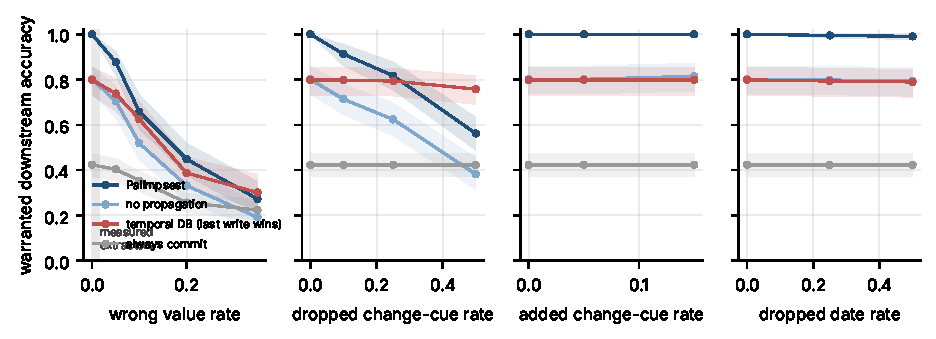
\includegraphics[width=\textwidth]{figures/noise.pdf}
\caption{Warranted downstream accuracy under injected extraction errors (mock extractor, 50 Setting 2 streams; bands are stream-level 95\% bootstrap intervals; the grey band marks the slot-error range of the real extractors, 0.3--1.5\%).}\label{fig:noise}
\end{figure}
Figure~\ref{fig:noise} injects extraction errors at controlled rates. \pal{} degrades faster than last-write-wins as wrong values accumulate: at 20\% wrong values it scores \nzSlotTwentyPal{} against \nzSlotTwentyTdb{} for the temporal DB and at 35\% the order reverses (\nzSlotThirtyfivePal{} vs \nzSlotThirtyfiveTdb); when half the stated change cues are dropped the temporal DB (\nzCueFiftyTdb) is ahead of \pal{} (\nzCueFiftyPal). Every extraction error becomes a standing dispute that the semantics keeps open, whereas last-write-wins discards it. The injected error types are the extractor's measured categories (wrong value, dropped cue, added cue, dropped date), but the rates at which the curves cross are far above the measured ones and are not deployment thresholds.

\subsection{Setting 3: streams derived from Wikidata revision histories}\label{sec:res-s3}
\begin{sidewaystable}\centering\footnotesize\setlength{\tabcolsep}{3.5pt}
\caption{Setting 3 (transfer: 30 streams assembled from Wikidata statement histories, pseudonymised surface, extraction and adjudication with Claude Haiku 4.5). Descriptive; the warranted-downstream stratum has 24 queries in 13 streams.}\label{tab:s3}
\begin{tabular}{lccccccc}
\toprule
System & Warr.\ downstream & Warr.\ direct & Resolvable & Unresolved & Commit rate$\downarrow$ & Prov.\ P & Cost (tok/stream) \\
\midrule
\textsc{Palimpsest} & 0.923 {\tiny[0.77,1.00]} & 0.976 {\tiny[0.94,1.00]} & 0.978 {\tiny[0.95,1.00]} & 0.909 {\tiny[0.73,1.00]} & 0.000 {\tiny[0.00,0.00]} & 0.892 {\tiny[0.85,0.94]} & 25k \\
\quad no propagation & 0.724 {\tiny[0.49,0.93]} & 0.976 {\tiny[0.94,1.00]} & 0.962 {\tiny[0.93,0.99]} & 0.879 {\tiny[0.70,1.00]} & 0.000 {\tiny[0.00,0.00]} & 0.886 {\tiny[0.84,0.93]} & 25k \\
\quad forced commit & 0.923 {\tiny[0.77,1.00]} & 0.976 {\tiny[0.94,1.00]} & 0.978 {\tiny[0.95,1.00]} & 0.000 {\tiny[0.00,0.00]} & 1.000 {\tiny[1.00,1.00]} & 0.892 {\tiny[0.85,0.94]} & 25k \\
Symbolic replay (rule adjudicator) & 0.923 {\tiny[0.77,1.00]} & 0.976 {\tiny[0.94,1.00]} & 0.978 {\tiny[0.95,1.00]} & 0.909 {\tiny[0.73,1.00]} & 0.000 {\tiny[0.00,0.00]} & 1.000 {\tiny[1.00,1.00]} & 25k \\
Claims log + LLM adjudicator & 0.019 {\tiny[0.00,0.06]} & 0.519 {\tiny[0.38,0.66]} & 0.185 {\tiny[0.14,0.23]} & 0.333 {\tiny[0.09,0.61]} & 0.545 {\tiny[0.27,0.79]} & 0.802 {\tiny[0.75,0.86]} & 88k \\
Raw-report log + LLM adjudicator (30 str.) & 0.077 {\tiny[0.00,0.23]} & 0.451 {\tiny[0.30,0.61]} & 0.181 {\tiny[0.13,0.23]} & 0.182 {\tiny[0.00,0.45]} & 0.576 {\tiny[0.30,0.82]} & 0.731 {\tiny[0.67,0.79]} & 71k \\
Claims log + LLM adj.\ (amended contract, 30 str.) & 0.019 {\tiny[0.00,0.06]} & 0.491 {\tiny[0.34,0.64]} & 0.205 {\tiny[0.15,0.26]} & 0.394 {\tiny[0.15,0.64]} & 0.485 {\tiny[0.21,0.73]} & 0.791 {\tiny[0.73,0.85]} & 92k \\
Raw-report log + LLM adj.\ (amended, 30 str.) & 0.173 {\tiny[0.00,0.38]} & 0.466 {\tiny[0.32,0.61]} & 0.208 {\tiny[0.15,0.26]} & 0.318 {\tiny[0.09,0.59]} & 0.439 {\tiny[0.18,0.70]} & 0.728 {\tiny[0.67,0.79]} & 25k \\
Temporal DB & 0.865 {\tiny[0.65,1.00]} & 0.884 {\tiny[0.78,0.97]} & 0.692 {\tiny[0.64,0.74]} & 0.000 {\tiny[0.00,0.00]} & 1.000 {\tiny[1.00,1.00]} & 0.922 {\tiny[0.88,0.96]} & 25k \\
Always abstain & 0.000 {\tiny[0.00,0.00]} & 0.000 {\tiny[0.00,0.00]} & 0.000 {\tiny[0.00,0.00]} & 0.788 {\tiny[0.55,1.00]} & 0.000 {\tiny[0.00,0.00]} & 0.828 {\tiny[0.78,0.88]} & 25k \\
Always commit & 0.000 {\tiny[0.00,0.00]} & 0.506 {\tiny[0.36,0.65]} & 0.478 {\tiny[0.43,0.53]} & 0.000 {\tiny[0.00,0.00]} & 0.909 {\tiny[0.73,1.00]} & 0.803 {\tiny[0.75,0.86]} & 25k \\
\bottomrule
\end{tabular}
\end{sidewaystable}
Setting 3 uses the only data in the study whose conflicts and withdrawals we did not generate: streams \emph{derived from independently authored Wikidata revision histories under an author-defined mapping}. Forty persons selected by a query for histories with deprecated statements and ended employments, and the 128 organisations recorded as their employers, were fetched (3{,}474 sampled revisions; intermediate edits between sampled revisions collapse into one diff) and mapped as follows: a claim added is an assertion (with a \emph{since} cue when it carries a start qualifier), a value edited in place is a correction, a statement deprecated or removed by the editors is a withdrawal; references give the source class (331 of 417 assertions are unreferenced, class \emph{low}); the surface is pseudonymised with the fictional names of Settings 1--2 and the dates are real. The target is editorial state, not the world: a deprecation is scored as a withdrawal of evidence, not as proof that a relationship ended. Three mappings were tried and are reported together: with \emph{employer} single-valued, 1 warranted downstream query in 30 streams; multi-valued and changeable, 4; multi-valued and stable (an affiliation set, which is what the property records), \sThreeWarrTotal{} in 13 streams. The third was adopted and frozen before the LLM runs; it is a consequential, author-made choice, and the setting is exploratory transfer. Two of the 128 organisations appear in more than one stream, so the streams are nearly disjoint and the stream-level bootstrap is appropriate.

\pal{} over the extracted claims reaches \sThreePalWarr{} on the \sThreeWarrTotal{} warranted downstream queries, equal to symbolic replay (\sThreeRuleWarr): the ceiling set by extraction (slot-error rate \sThreeExtSlot\%). Removing propagation costs $\sThreeProp$ points $[\sThreePropLo, \sThreePropHi]$ over 13 streams, a suggestive rather than broad confirmation. The LLM adjudicator reaches \sThreeLogWarr{} on the same queries and \sThreeLogRes{} on resolvable ones under the original contract, and \sThreeCtwoLogWarr{} and \sThreeCtwoLogRes{} under the amended one, so the missing convention explains little of this gap; what does is that \sThreeEstEmpty{} of the \sThreeEstTotal{} established primary queries are empty sets and \sThreeHoldsFalse{} are established-false, on which it answers \emph{unknown}, and that on the warranted queries it answers \emph{unresolved} with the gold set among its alternatives, reasoning that overlapping affiliations ``may have ended'' against a schema that declares the attribute stable. The pseudonymised schema puts the adjudicator's priors against a declaration it was told to follow; that is a limitation of this transfer design as much as of the adjudicator, and the propagation ablation and the equality with replay are the parts of Setting 3 we would rely on.

\subsection{External check: LongMemEval knowledge updates}\label{sec:res-lme}
\begin{table}[t]\centering\footnotesize
\caption{LongMemEval knowledge-update items (78; 69 mapped to an extracted attribute). Systems answer one structured slot from claims extracted turn by turn; a Haiku judge compares the answer with the reference. Coverage = share answered as established; accuracy over all items and over answered items. Not comparable to published LongMemEval scores.}\label{tab:lme}
\begin{tabular}{lccc}
\toprule
System & Coverage & Acc.\ (all) & Acc.\ (answered) \\
\midrule
\pal{} (P0c) & 0.32 & 0.167 & 0.400 \\
\pal{} + self-update (exploratory) & 0.74 & 0.474 & 0.621 \\
Temporal DB (last write wins) & 0.88 & 0.526 & 0.594 \\
Always-commit & 0.88 & 0.526 & 0.594 \\
Always-abstain & 0.00 & 0.038 & 0.000 \\
Claims log + LLM adjudicator & 0.56 & 0.359 & 0.614 \\
\bottomrule
\end{tabular}
\end{table}
LongMemEval's knowledge-update items \citep{longmemeval} ask for a user attribute stated and later updated across chat sessions. We run the \lmeN{} items of the oracle release (cleaned version of 3 October 2026; sessions are not chronologically ordered in the release and are sorted by their timestamps before belief time is assigned) through an open-vocabulary adapter shared by all systems: each user turn is extracted into claims about the user, attribute keys are canonicalised per item, the question is mapped to one key, every system answers that slot, and a model judge compares the answer with the reference; abstention is credited on the six items whose reference is ``not enough information''. The adapter caps every system (9 items map to no key; always-abstain scores 3/78 because three abstention items are among the unmapped) and the numbers are not comparable to published LongMemEval scores.

Two things are measured at once and we separate them. The benchmark's reference for an update is the user's \emph{latest} statement: it tests the self-update regime of Table~\ref{tab:regime} and only that regime. Under P0c a later uncued value from the same source is a dispute, so \pal{} answers \emph{unresolved} on \lmePalUnres{} of 69 mapped items (coverage \lmePalCov, accuracy \lmePalAcc), where last-write-wins answers and is right on 34 of them (\lmeTdbAcc{} at coverage \lmeTdbCov); on items where both commit they agree, and support-ranked commitment reproduces last-write-wins exactly, because with a single source support reduces to recency. The adapter is the other limit: the extractor recovered a stated change on 5 of 91 claims on the queried keys, questions about previous values or about the change itself cannot be expressed in a single current-value slot, and the LLM adjudicator abstains on 44\% (\lmeLogAcc). The pre-registered self-update rule, applied to these already-seen items as a mechanism check only, gives \lmePalSuAcc{} at coverage \lmePalSuCov. Our reading: a policy that requires explicit change cues loses coverage wherever updates arrive as ordinary self-reports, which is a practical limitation of P0c and the reason A-SU is now the default for self-report streams; and what this benchmark does not contain---unreliable sources, hidden world state, withdrawn evidence---is what the other settings measure. STALE \citep{stale2026} was not evaluated: at the time of our runs we could not reach a data release, and its native question interface at 100K-token contexts exceeded the remaining budget; a public repository has since been reported and the evaluation is left for a later version.

\subsection{Calibrated support and poisoning}\label{sec:res-rq3}
\begin{table}[t]\centering\small
\caption{RQ3, Setting 1 (held-out streams): claim-level calibration of support against the hidden world. Lower is better.}\label{tab:rq3}
\begin{tabular}{lccc}
\toprule
Confidence & Brier & ECE & AURC \\
\midrule
Evidence model, declared priors & 0.182 & 0.118 & 0.138 \\
Evidence model, learned class priors & 0.175 & 0.113 & 0.131 \\
\quad without origin grouping & 0.179 & 0.121 & 0.136 \\
\quad without recency & 0.236 & 0.202 & 0.156 \\
\quad without cue adjustments & 0.183 & 0.128 & 0.136 \\
Class prior only & 0.255 & 0.227 & 0.168 \\
Logistic regression on evidence features & 0.138 & 0.034 & 0.112 \\
Constant 0.5 & 0.250 & 0.496 & 0.268 \\
\bottomrule
\end{tabular}
\end{table}
Support (\S\ref{sec:support}) is a weighted log-odds rule, auditable but not a fitted model, and it predicts a defined event: that a candidate value is the world value at the query's valid time. On 200 held-out Setting 1 streams (\RqN{} candidate values) with class priors learned on 300 training streams it has ECE \RqLearnedEce{} and Brier \RqLearnedBrier, against \RqPriorEce{} and \RqPriorBrier{} for class priors alone, and against \RqLogregEce{} and \RqLogregBrier{} for a logistic regression over the same evidence features trained on the same streams; recency is the largest single contributor (ECE \RqNoRecEce{} without it). In Setting 2, on the \RqTwoSupN{} value queries the LLM adjudicator answered as established and the same asserted values, support has ECE \RqTwoSupEce{} against \RqTwoVerbEce{} for the adjudicator's verbalised confidence and \RqTwoSampEce{} for agreement across five samples on a 300-query subset (risk--coverage areas \RqTwoSupAurc, \RqTwoVerbAurc, \RqTwoSampAurc). H3 is not supported: a provenance-and-recency rule is less well calibrated than a learned predictor and than the adjudicator's own confidence on these populations. The selection by the adjudicator's established answers and the smaller sampling subset are reported as such; reliability diagrams are in Appendix~\ref{app:tables} (Figure~\ref{fig:rel}).
\begin{table}[t]\centering\small
\caption{Poisoning (Setting 1, 60 streams per cell). Attacker injects false assertions at a rate of the honest ones, half with a false change cue; harm = share of value queries answered \emph{established} with the poisoned value; support = mean support the evidence model assigns to poisoned vs.\ honest candidates.}\label{tab:poison}
\begin{tabular}{llcccccc}
\toprule
Channel & Rate & \multicolumn{2}{c}{\textsc{Palimpsest}} & \multicolumn{2}{c}{Temporal DB} & \multicolumn{2}{c}{Support} \\
 & & harm$\downarrow$ & unresolved & harm$\downarrow$ & unresolved & poisoned & honest \\
\midrule
low & 0.01 & 0.003 & 0.27 & 0.003 & 0.03 & 0.21 & 0.67 \\
low & 0.05 & 0.024 & 0.28 & 0.030 & 0.03 & 0.33 & 0.67 \\
low & 0.20 & 0.112 & 0.30 & 0.151 & 0.03 & 0.32 & 0.65 \\
trusted & 0.01 & 0.005 & 0.27 & 0.005 & 0.03 & 0.63 & 0.67 \\
trusted & 0.05 & 0.027 & 0.28 & 0.033 & 0.03 & 0.66 & 0.66 \\
trusted & 0.20 & 0.115 & 0.30 & 0.153 & 0.03 & 0.63 & 0.63 \\
\bottomrule
\end{tabular}
\end{table}
Under the explicit attacker model (Table~\ref{tab:poison}), at 20\% injection through a low-trust channel \pal{} answers established with the poisoned value on \PoisHarmPal\% of value queries against \PoisHarmTdb\% for the temporal DB, and the support layer separates poisoned from honest candidates through the low channel (mean support \PoisSupLowPois{} vs \PoisSupLowHon) but not through a compromised trusted one (\PoisSupTrPois{} vs \PoisSupTrHon): provenance cannot detect what provenance has endorsed. The regime view (\S\ref{sec:res-regime}) adds the conditional number: when the latest report is the injection, \pal{} commits to the injected value on \rgPoisPalInj{} of queries.


\section{Threats to validity}\label{sec:threats}
\paragraph{Construct.} The generator, the semantics and the system share an author; Settings 1--2 could be tuned to the method. The pre-registered selection rule, the declared perturbation menu, the sensitivity variants, the equivalence with symbolic replay (which shares the per-key oracle) and the brute-force global oracle check of Appendix~\ref{app:semantics} (a separate implementation) are the defence we offer; the transfer setting is independent in its data, not in its mapping, and the mapping was reached after two alternatives left the target stratum nearly empty. The semantics embodies choices a reader may reject: inertia, report-time anchoring, closed-world yes/no answers, the empty-set convention, and above all cue resolution (A-CUE), adopted after literal P0 left the benchmark abstention-dominated and shown by the poisoning regime to be an attack surface. The dependency structure is a fixed, declared rule schema given to every system; nothing here extracts rules from text.

\paragraph{Internal.} The LLM comparisons change who reasons and when at once; the replay row separates the two, and the systems benchmark answers the when-question without an LLM. The contract as run lacked the empty-set convention; the amended-contract reruns on the common subset bound its effect. LLM prompts were developed on five development streams only and not tuned; a better-prompted adjudicator would score higher, and the Sonnet subset shows how much the gap depends on the model. The ``unsupported propagation'' endpoint as registered conflated harmful and harmless answer changes; the transition table replaces it for the harm claim.

\paragraph{Statistical.} The stream is the unit; intervals are cluster bootstraps. The primary estimate uses 99 of 100 streams (one has no warranted downstream query); the Setting 3 propagation estimate rests on 24 queries in 13 streams; the LongMemEval numbers have no intervals and should be read as counts. Holm correction was declared for H2--H4 and is applied in Appendix~\ref{app:tables} (Table~\ref{tab:holm}) with one-sided stream-level bootstrap $p$-values (10{,}000 resamples): H2 ($r^*<1$) $p<10^{-4}$, H4 (both components) $p<10^{-4}$, H3 (lower ECE) $p=\holmHThree$; Holm-adjusted, H2 and H4 are rejected at $\alpha=0.05$ and H3 is not.

\paragraph{External.} One backbone family at full scale; fictional entity names remove world knowledge, a deliberate control that in Setting 3 put the adjudicator's priors against the declared schema. No independent human audit of paraphrases, extractions or judge decisions was performed; the same model family produced and checked them. LongMemEval tests the self-update regime only, STALE was not evaluated, and the seven-reports-per-key cap of the main generator configuration bounds the oracle's enumeration in Settings 1--3 (the scale sweep of \S\ref{sec:res-systems} relaxes it to 10 and 13).

\paragraph{Budget.} The whole study ran under a \$100 ceiling (measured spend \$\spendTotal); Setting 2 has 100 streams rather than the registered 150, the LLM baselines on the amended contract have 30, and the external checks are subsamples.


\section{Conclusion}
We asked a narrow question with instruments built so that the easy failure modes do not pay: a semantics of justified belief that keeps alternatives open, a contract that scores behaviour rather than representation, and a benchmark in which the world, the reports and what the reports justify are separable. The results are these. Retraction propagation through justifications, not ordinary belief updating, prevents downstream errors, by about twenty points in every setting including real revision histories. An incremental store that pins justifications returns the same status, value and alternatives as a symbolic replay does, with lower measured query latency, and saves total work only when queries are at least as frequent as observations or histories are long; its write cost grows exponentially in reports per key. Symbolic maintenance beats a prompted LLM adjudicator over the same extracted claims by a wide margin, but a rule-based adjudicator over the same claims does as well, so that result is about the adjudicators, not about write time. Refusing to assume recency buys protection exactly where the latest report is wrong, and costs abstention where it is right, which is most of the time in our generator and all of the time in a self-report benchmark; a pre-registered same-origin self-update rule closes the single-source case at a measured cost of at most 1.3 points of wrong commitments where the latest report is wrong. The evidence model's support is a defined, auditable quantity and not a better-calibrated or a better-committing one than simpler alternatives, and when the latest report is an injection the store commits to it on \rgPoisPalInj{} of queries, little less than recency. Everything needed to reproduce, contest or extend these results is released with the dated pre-registration and the cost ledger.


\bibliographystyle{plainnat}
\bibliography{refs}

\appendix
\section{Semantics: conventions, totality and corner cases}\label{app:semantics}
\paragraph{Conventions.} Belief time is the report day; two reports on the same day are ordered by id, and a query at belief time $\tau$ sees every report with $t_{\mathrm{rep}}\le\tau$. A report with no temporal cue is anchored at its report day; \texttt{since}~$t$ anchors it at $t$ (which may precede the report day); \texttt{at}~$t$ asserts the value at $t$ only. A query before the first anchor on a key is \texttt{unknown}; a query inside a gap between two different accepted anchors on a single-valued key has both neighbours as candidates (unknown change point); a reversal is two changes. Withdrawn evidence is never restored. A correction whose target is absent from the stream is an ordinary assertion; a correction of a withdrawn report is accepted and has no further effect; a same-origin correction later withdrawn leaves its target withdrawn (withdrawal is not undone); a source withdrawal removes every report of that source, including reports it makes after the withdrawal, for all later belief times. Multi-valued \texttt{competing\_values=false} attributes never dispute; their runs end only through withdrawal or correction.

\paragraph{Decision table: unknown, empty, false.} The three conventions of \S\ref{sec:semantics} applied to the cases a reader asked about (verified on toy streams in \texttt{tests/}):

\begin{center}\small\begin{tabular}{lccc}\toprule
Situation at the query & single-valued slot & multi-valued slot & yes/no ``holds $v$'' \\\midrule
no report on the key & \texttt{unknown} & \texttt{established} $\emptyset$ & \texttt{established} false \\
every report on the key withdrawn & \texttt{unknown} & \texttt{established} $\emptyset$ & \texttt{established} false \\
belief time before the first report & \texttt{unknown} & \texttt{established} $\emptyset$ & \texttt{established} false \\
undeclared entity or attribute & \texttt{unknown} & \texttt{unknown} & \texttt{unknown} \\
ladder exhausted (every report rejected) & \texttt{unknown} & \texttt{unknown} & \texttt{unknown} \\
$v$ never asserted, key otherwise established & \texttt{established} $\neq v$ & set without $v$ & \texttt{established} false \\\bottomrule
\end{tabular}\end{center}
The first three rows have exactly one admissible interpretation with an empty timeline, which yields no candidate for a single-valued slot (hence \texttt{unknown}), the empty set for a multi-valued slot, and falsity for every ``holds'' proposition (closed world over admitted evidence); the undeclared and ladder-exhausted rows have no interpretation, hence \texttt{unknown} throughout. The difference between a missing key and an exhausted ladder is reported through the ladder counter, not through the status.

\paragraph{Relaxation ladder (totality).} The per-key enumeration can leave a key with no admissible interpretation on extracted or adversarial streams (e.g.\ a change presupposition whose only witness is withdrawn, or under P1). The oracle is made total by a declared ladder applied per key only when the admissible set is empty: (1) drop A-CHG presuppositions; (2) additionally fall back to literal P0 dispute (no cue shielding); (3) reject every report on the key (status \texttt{unknown}). Each application is counted; the ladder never fired on the 500 generated Setting 1 streams under P0c, on the 100 extracted Setting 2 streams, or on the 30 Setting 3 streams (counted on 3 October 2026).

\paragraph{Rules and the per-key factorisation.} Derived attributes are forward-chained per interpretation; the released domains are acyclic with derivation depth $\le2$, and cyclic rule sets are outside the declared scope. A defeasible rule contributes nothing under an interpretation in which its exception holds (explicit truth of the exception, not absence). A derived value with several independent derivations keeps its candidate when one premise is withdrawn as long as another derivation survives; provenance records every derivation path that yields a candidate. The oracle computes interpretation sets \emph{per key} and lets the rule engine branch over the per-key candidate unions. This is exact, not an approximation, under two conditions that the declared semantics and rule sets satisfy: (i) every admissibility condition (A-ERR, A-CORR, A-CHG, A-CUE, A-CONS, A-SU) relates reports on the same key, and a correction that refers to a report on another key acts only through admission (A-SELF withdrawal), so the set of global interpretations is the Cartesian product of the per-key sets; (ii) no key occurs more than once on a derivation path, so a derived candidate obtained from one candidate per key is realised by the global interpretation that picks those per-key interpretations. An earlier draft of this appendix said that the factorisation ``can over-generate alternatives'' in general; the correct statement is that it over-generates exactly when condition (ii) fails. The reviewer's diagnostic shows it: with $U\leftarrow X$, $V\leftarrow X$ and $W\leftarrow U\wedge V$ and $X$ unresolved between $A$ and $B$, the global semantics gives $W\in\{A,B\}$ while the per-key procedure also produces the impossible mixed derivation (reported as a ``no value'' alternative); the released check reproduces this (\texttt{oracle\_validation.py --counterexample}) and a static test on the rule sets (the attribute closures of a rule's body atoms must be pairwise disjoint) flags that domain and passes every released domain. Independent alternative proofs of one derived value do not occur in the released rule sets (one rule per derived attribute), and the validation below covers defeasible exceptions and multi-valued alternatives through the generator's own domain. Validation (\texttt{scripts/oracle\_validation.py}): on \ovStreams{} streams (the three hand-written references and 300 small generated ones, seeds 40000--) and every value query whose dependency closure admits at most \ovMaxEnum{} reports (\ovSkipped{} larger closures skipped), the per-key gold was compared with a brute-force \emph{global} computation that enumerates every TRUE/ERR and CONT/ENDED labelling of the closure's reports and derives each query under each global interpretation's own timelines for all keys at once: \ovQueries{} value queries (\ovDerived{} on derived slots), \ovDisagree{} disagreements in status, value or alternative set; the product structure $|\text{global}|=\prod_{\text{keys}}|\text{per-key}|$ held in all \ovQueries{} checks, and the per-key gold on the closure sub-stream equalled that on the full stream in every case (\ovClosureFail{} failures), which is the independence of keys outside the closure.

\paragraph{Worked example, revisited (reviewer question).} With \emph{residence} multi-valued and changeable, after ``Alex lives in London'' (o1) and ``Alex moved from London to Paris'' (o2), A-CHG requires some earlier London report to be accepted, A-CUE shields o2 from o1, and the \textsc{ended} label on London's run is \emph{forced} by the \emph{from} clause of the change cue (\S\ref{sec:semantics}, ``a change-from cue forces \textsc{ended} on the run of the previous value''); the written clause of the earlier draft omitted this sentence and the implementation has always had it. Without the \emph{from} clause (``Alex has moved to Paris'') London's continuation stays open, and ``Did Alex move?'' is \texttt{established} while ``Does Alex still live in London?'' is \texttt{possible}.


\section{Additional tables}\label{app:tables}
\begin{table}[t]\centering\small
\caption{Setting 1: exact accuracy by query slot (mean over 500 streams).}\label{tab:slots}
\begin{tabular}{lcccccc}
\toprule
Slot & \textsc{Palimpsest} & no propagation & forced commit & Temporal DB & Always commit & Always abstain \\
\midrule
as-of valid time & 1.000 & 1.000 & 0.743 & 0.653 & 0.638 & 0.168 \\
as-of belief time & 1.000 & 1.000 & 0.808 & 0.777 & 0.782 & 0.223 \\
current & 1.000 & 1.000 & 0.723 & 0.675 & 0.701 & 0.242 \\
downstream (derived) & 1.000 & 0.870 & 0.664 & 0.578 & 0.296 & 0.000 \\
reported & 1.000 & 1.000 & 1.000 & 1.000 & 1.000 & 1.000 \\
changed? & 1.000 & 1.000 & 0.932 & 0.919 & 0.919 & 0.068 \\
erroneous? & 1.000 & 1.000 & 0.704 & 0.001 & 0.001 & 0.296 \\
holds at $t$? & 1.000 & 1.000 & 0.877 & 0.771 & 0.734 & 0.224 \\
\bottomrule
\end{tabular}
\end{table}
Table~\ref{tab:slots} breaks Setting 1 accuracy down by slot: systems without justifications fail on \emph{erroneous?} almost completely, lose most on downstream slots, and answer as-of-belief-time questions from the current state.
\begin{table}[t]\centering\small
\caption{Sensitivity of the Setting 1 gate to the dispute semantics (500 streams). Warranted downstream queries per stream, and the propagation on$-$off difference on them.}\label{tab:sens}
\begin{tabular}{lcccc}
\toprule
Policy & warr./stream & \textsc{Palimpsest} & no propagation & Temporal DB \\
\midrule
P0c (main) & 7.42 & 1.000 {\tiny[1.00,1.00]} & 0.794 {\tiny[0.78,0.81]} & 0.807 {\tiny[0.79,0.82]} \\
literal P0 & 3.38 & 1.000 {\tiny[1.00,1.00]} & 0.638 {\tiny[0.61,0.67]} & 0.918 {\tiny[0.90,0.93]} \\
P1 & 3.49 & 1.000 {\tiny[1.00,1.00]} & 0.688 {\tiny[0.66,0.72]} & 0.866 {\tiny[0.84,0.89]} \\
\bottomrule
\end{tabular}
\end{table}
Table~\ref{tab:sens}: under literal P0 a stream yields \sOneLitPZeroWarr{} warranted downstream queries and the propagation effect is $+\sOneLitPZeroEffect$ points; under P1, \sOnePOneWarr{} and $+\sOnePOneEffect$. The qualitative conclusion does not depend on the policy; the size of the usable stratum does.
\begin{sidewaystable}\centering\footnotesize\setlength{\tabcolsep}{3.5pt}
\caption{Sign-stability subset: 15 Setting 2 streams re-extracted and adjudicated with Claude Sonnet 4.6 on the same frozen evaluation set.}\label{tab:s2strong}
\begin{tabular}{lccccccc}
\toprule
System & Warr.\ downstream & Warr.\ direct & Resolvable & Unresolved & Commit rate$\downarrow$ & Prov.\ P & Cost (tok/stream) \\
\midrule
\textsc{Palimpsest} & 1.000 {\tiny[1.00,1.00]} & 1.000 {\tiny[1.00,1.00]} & 1.000 {\tiny[1.00,1.00]} & 0.816 {\tiny[0.73,0.90]} & 0.090 {\tiny[0.05,0.14]} & 0.987 {\tiny[0.98,1.00]} & 189k \\
\quad no propagation & 0.780 {\tiny[0.64,0.90]} & 1.000 {\tiny[1.00,1.00]} & 0.946 {\tiny[0.91,0.98]} & 0.805 {\tiny[0.72,0.89]} & 0.090 {\tiny[0.05,0.14]} & 0.984 {\tiny[0.97,0.99]} & 189k \\
\quad forced commit & 1.000 {\tiny[1.00,1.00]} & 1.000 {\tiny[1.00,1.00]} & 1.000 {\tiny[1.00,1.00]} & 0.048 {\tiny[0.00,0.12]} & 0.751 {\tiny[0.62,0.87]} & 0.989 {\tiny[0.98,1.00]} & 189k \\
Symbolic replay (rule adjudicator) & 1.000 {\tiny[1.00,1.00]} & 1.000 {\tiny[1.00,1.00]} & 1.000 {\tiny[1.00,1.00]} & 0.816 {\tiny[0.73,0.90]} & 0.090 {\tiny[0.05,0.14]} & 0.997 {\tiny[0.99,1.00]} & 189k \\
Claims log + LLM adjudicator & 0.813 {\tiny[0.67,0.93]} & 0.924 {\tiny[0.85,0.98]} & 0.854 {\tiny[0.80,0.91]} & 0.289 {\tiny[0.19,0.39]} & 0.489 {\tiny[0.36,0.63]} & 0.851 {\tiny[0.82,0.88]} & 718k \\
Temporal DB & 0.777 {\tiny[0.64,0.89]} & 0.844 {\tiny[0.67,0.97]} & 0.908 {\tiny[0.86,0.95]} & 0.000 {\tiny[0.00,0.00]} & 0.833 {\tiny[0.72,0.92]} & 0.957 {\tiny[0.94,0.97]} & 189k \\
Always abstain & 0.000 {\tiny[0.00,0.00]} & 0.000 {\tiny[0.00,0.00]} & 0.000 {\tiny[0.00,0.00]} & 0.399 {\tiny[0.30,0.49]} & 0.000 {\tiny[0.00,0.00]} & 0.531 {\tiny[0.47,0.58]} & 189k \\
Always commit & 0.387 {\tiny[0.29,0.48]} & 0.990 {\tiny[0.97,1.00]} & 0.778 {\tiny[0.72,0.83]} & 0.000 {\tiny[0.00,0.00]} & 0.879 {\tiny[0.84,0.92]} & 0.945 {\tiny[0.92,0.97]} & 189k \\
\bottomrule
\end{tabular}
\end{sidewaystable}
\begin{table}[t]\centering\small
\caption{RQ2 corruption curve (50 Setting 2 streams, mock extractor with injected error rates). Warranted downstream accuracy; PALIMPSEST resolvable and unresolved accuracy.}\label{tab:noise}
\begin{tabular}{llcccccc}
\toprule
Error type & rate & \textsc{Palimpsest} & no prop. & Temporal DB & Always commit & PAL resolvable & PAL unresolved \\
\midrule
wrong value & 0.00 & 1.000 & 0.801 & 0.799 & 0.423 & 1.000 & 1.000 \\
wrong value & 0.05 & 0.878 & 0.706 & 0.738 & 0.404 & 0.910 & 0.858 \\
wrong value & 0.10 & 0.658 & 0.519 & 0.625 & 0.354 & 0.814 & 0.685 \\
wrong value & 0.20 & 0.449 & 0.332 & 0.388 & 0.257 & 0.652 & 0.515 \\
wrong value & 0.35 & 0.273 & 0.192 & 0.301 & 0.224 & 0.511 & 0.347 \\
change cue dropped & 0.10 & 0.912 & 0.713 & 0.797 & 0.423 & 0.946 & 0.958 \\
change cue dropped & 0.25 & 0.817 & 0.624 & 0.794 & 0.423 & 0.867 & 0.873 \\
change cue dropped & 0.50 & 0.562 & 0.382 & 0.758 & 0.423 & 0.712 & 0.753 \\
change cue added & 0.05 & 1.000 & 0.801 & 0.799 & 0.423 & 1.000 & 0.963 \\
change cue added & 0.15 & 1.000 & 0.815 & 0.799 & 0.423 & 1.000 & 0.871 \\
date dropped & 0.25 & 0.995 & 0.798 & 0.794 & 0.423 & 0.995 & 0.973 \\
date dropped & 0.50 & 0.991 & 0.794 & 0.790 & 0.423 & 0.990 & 0.961 \\
\bottomrule
\end{tabular}
\end{table}
\begin{table}[t]\centering\small
\caption{Regime table on the 500 frozen Setting 1 streams (P0c; same definitions as Table~\ref{tab:regime}).}\label{tab:regime-s1}
\begin{tabular}{lrccccc}
\toprule
Regime & $n$ & LWW & valid & P0c world & P0c abst. & P0c wrong commit \\
\midrule
self-update & 50 & 0.92 & 0.92 & 0.78 & 0.20 & 0.02 \\
multi-source update & 1504 & 0.92 & 0.91 & 0.69 & 0.27 & 0.04 \\
earlier report erroneous & 2376 & 0.92 & 0.90 & 0.51 & 0.45 & 0.04 \\
delayed report & 159 & 0.08 & 0.42 & 0.14 & 0.65 & 0.21 \\
latest erroneous, low-trust & 364 & 0.04 & 0.10 & 0.02 & 0.92 & 0.07 \\
latest erroneous, other & 234 & 0.06 & 0.13 & 0.03 & 0.91 & 0.06 \\
latest withdrawn & 463 & 0.49 & 0.49 & 0.35 & 0.35 & 0.30 \\
no conflict & 1615 & 0.64 & 0.64 & 0.64 & 0.09 & 0.27 \\
\bottomrule
\end{tabular}
\end{table}
\begin{table}[t]\centering\small
\caption{Registered secondary hypotheses with one-sided stream-level cluster-bootstrap $p$-values (10{,}000 resamples) and Holm correction over the family $\{$H2, H3, H4$\}$; H4 uses the larger of its two components. Estimates are paired per-stream differences (H4) or the statistic itself (H2: $r^*$; H3: ECE(support) $-$ ECE(verbalised)).}\label{tab:holm}
\begin{tabular}{llccc}
\toprule
Hypothesis & Statistic & Estimate [95\% CI] & $p$ (one-sided) & Holm-adjusted \\
\midrule
H2 & $r^*<1$ & 0.228 [0.224, 0.233] & $<10^{-4}$ & $<10^{-4}$ \\
H3 & ECE difference $<0$ & 0.062 [0.015, 0.078] & 0.998 & 0.998 \\
H4a & commit-rate difference $<0$ & -0.492 [-0.533, -0.451] & $<10^{-4}$ & \multirow{2}{*}{$<10^{-4}$} \\
H4b & resolvable difference $\ge -0.03$ & 0.310 [0.286, 0.333] & $<10^{-4}$ & \\
\bottomrule
\end{tabular}
\end{table}
\begin{figure}[t]\centering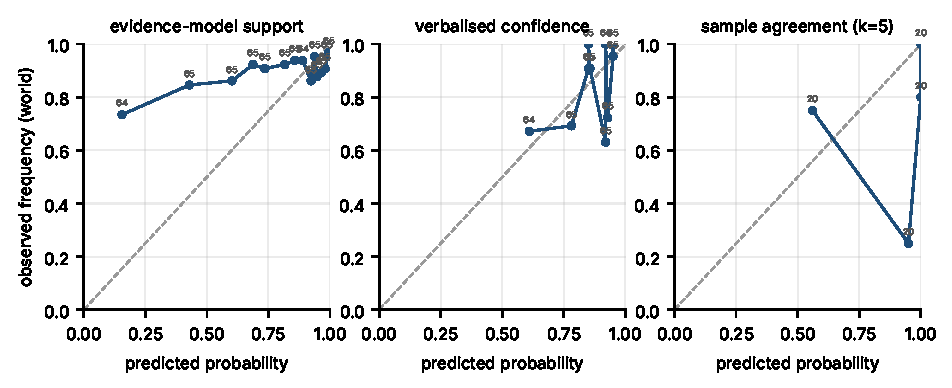
\includegraphics[width=\textwidth]{figures/reliability.pdf}
\caption{Reliability diagrams on the \RqTwoSupN{} Setting 2 value queries the LLM adjudicator answered as established (15 equal-mass bins; bin counts annotated; the sampling comparator uses its 300-query subset).}\label{fig:rel}
\end{figure}

\section{Error taxonomy of the LLM adjudicator (Setting 2)}\label{app:errors}
Rule-coded categories over the 4{,}062 primary answers (non-companion, non-\texttt{reported}) of the claims-log LLM adjudicator, original protocol, against the frozen gold (\texttt{data/s2/\_error\_taxonomy\_llm.json}): correct 47.7\%; premature commitment on an unresolved or possible slot 15.7\%; under-commitment on an established slot with the gold value among the listed alternatives 9.8\%, and with it absent 1.0\%; wrong alternative set on an unresolved slot 8.2\%; wrong committed value 6.0\%; an answer on a slot whose gold is \texttt{unknown} 6.5\%; \texttt{unknown} on an established slot 1.6\%; convention cases 3.0\% in total (empty-set gold 1.1\%, established-false gold 1.9\%; the categories are exclusive, assigned in the order listed); status confusion and other 0.4\%. The coding is by rule, not by a blinded human; it separates commitment errors from convention errors and from value errors, which is what the main text uses.

\section{Prompts and contract}\label{app:prompts}
\subsection*{Shared output contract, amended version (contract/shared\_prompt.md); the original-protocol version is the same text without the marked clarification (contract/shared\_prompt\_original.md)}
{\scriptsize\begin{verbatim}
# Shared answering instruction (v0.1) — identical for every system

You answer questions about an entity-attribute world from a stream of observations.
Observations may conflict, arrive late, come from unreliable sources, or be retracted. You will
be given: the vocabularies (entities, attributes with their value types, cardinality and
whether they can change), the normalisation rules, the observations or memory available to you
(each with an observation id), and one query with its answer slot.

Your job is to report what the admitted observations **justify**, not what you guess is true.
When the observations do not uniquely determine the answer, preserve that uncertainty. You may
assert what holds under every admissible reading of the evidence; you must qualify, list
alternatives, or abstain on anything that differs between readings. Picking one reading when
the evidence does not force it is an error.

## Output

Return exactly one JSON object and nothing else:

```json
{"query_id": "...", "status": "established|possible|unresolved|unknown",
 "assertion": <value|list|boolean|object|null>, "alternatives": [...],
 "provenance": ["o12", "o15"], "explanation": "optional, max 600 chars"}
```

## Status — definitions

- `established`: the assertion holds under **every** admissible reading of the admitted
observations, given the declared assumptions. This is about justification, not independently
verified truth. A yes/no proposition that is false under every reading is `established` with
`assertion: false`.
- `possible`: a **single** proposition holds under some readings but not all. Use for yes/no
questions and for single claims the evidence permits but does not force. `assertion` is that
proposition (for yes/no: `true`).
- `unresolved`: the question asks for a value and the admissible readings give **different**
values. List every candidate in `alternatives` (sorted; use `null` for "no value" when some
reading yields none; for multi-valued attributes each candidate is a sorted list) and set
`assertion` to `null`. The difference from `possible`: `possible` qualifies one claim;
`unresolved` declines to choose between claims.
- For a **multi-valued** attribute the answer is the sorted list of justified values; when
every admissible reading justifies no value at all (nothing reported, or everything reported
withdrawn), the answer is `established` with the empty list `[]`, not `unknown`. (`unknown` is
for single-valued slots with no candidate and for questions about undeclared entities or
attributes.) *[Clarification added 3 Oct 2026 after the original-protocol runs, which used the
contract without this sentence (archived as contract/shared_prompt_original.md); the amended-
protocol reruns on the 30-stream subset and Setting 3 used this version.]*
- `unknown`: no admitted observation bears on the question at all. Distinct from `unresolved`,
which has candidates.

## Rules of justification you must apply

1. A value reported with no date is taken to have held at least at the time of the report, and
to persist until a later report of a different value.
2. Two reports of different values for a single-valued attribute may be a change over time
**or** an error in one of them; both readings are admissible unless a report says which (a
stated change, or a stated correction). Do not assume a report is wrong merely because its
source is less reliable; do not assume it is right merely because it is newer.
3. For a multi-valued attribute (e.g. a person may have several residences), two different
reported values may both hold; the earlier one may also have ended, or either report may be in
error, as declared by that attribute's rules.
4. A retracted observation (or all observations from a retracted source) is withdrawn: nothing
may rely on it, and any conclusion that depended only on it loses its support.
5. A derived attribute follows from its rule only when the rule's conditions hold and no
declared exception holds.
6. Asked what you believed at an earlier time, answer from the observations available then.

## Examples (declared: `residence` is multi-valued, changeable, and differing residence reports
count against each other)

Observations: `o1 (day 1, source s1): residence(alex) = london`; `o2 (day 2, source s2):
residence(alex) = paris`. No dates, no statement of change or correction.

| Query | Answer |
|---|---|
| Did Alex move from London to Paris? | `{"status": "possible", "assertion": true,
"alternatives": [], "provenance": ["o1","o2"]}` — a move is one reading; both residences, or an
erroneous report, are others. |
| Was the London report wrong? | `{"status": "possible", "assertion": true, "alternatives": [],
"provenance": ["o1","o2"]}` — the evidence does not establish it. |
| What residences have been reported for Alex? | `{"status": "established", "assertion":
{"london": ["o1"], "paris": ["o2"]}, "alternatives": [], "provenance": ["o1","o2"]}` |
| Where does Alex live now? | `{"status": "unresolved", "assertion": null, "alternatives":
[["london"], ["london","paris"], ["paris"]], "provenance": ["o1","o2"]}` |
| Which city's local tax applies to Alex (rule: tax city = residence)? | `{"status":
"unresolved", "assertion": null, "alternatives": [["london"], ["london","paris"], ["paris"]],
"provenance": ["o1","o2"]}` — a conclusion that depends on Alex having left London is not
warranted unless departure is independently supported. |

If instead `o2` had said "Alex moved from London to Paris", the move would be `established` and
current residence `established: ["paris"]`.

## Provenance

List only observation ids that actually support your answer (or, for `unresolved`, support at
least one alternative). Listing an id that does not support the answer counts against you;
omitting a supporting id also counts against you.

## Formatting

Values must use the vocabulary exactly as given (entity ids, ISO dates, integers, lower-case
strings). Output the JSON object only — no prose before or after it.
\end{verbatim}}

\subsection*{Repair prompt (contract/repair\_prompt.md)}
{\scriptsize\begin{verbatim}
# Repair instruction (v0.1) — identical for every system, used at most once per answer

The previous output did not validate against the required schema. Reproduce the **same answer**
as a single valid JSON object with exactly these keys: `query_id` (string), `status` (one of
`established`, `possible`, `unresolved`, `unknown`), `assertion` (value, sorted list, boolean,
object, or null), `alternatives` (array, empty unless status is `unresolved`), `provenance`
(array of observation id strings, no duplicates), and optionally `explanation` (string <= 600
characters). Do not change the substance of the answer. Output the JSON object only.

Validation error: {{error}}

Previous output:
{{raw}}
\end{verbatim}}

\subsection*{Extractor system prompt (nl/extractor.py)}
{\scriptsize\begin{verbatim}
You convert one news-style report about people and organisations into a structured claim.
Output exactly one JSON object and nothing else:
{"kind": "assert" | "retract",
 "entity": <entity id>, "attr": <attribute>, "value": <value>,
 "valid": {"cue": "none" | "since" | "at", "date": "YYYY-MM-DD" or null},
 "op_cue": "none" | "change" | "correction", "op_from": <previous value or null>, "op_of":
<report id or null>,
 "target": <report id or source key or null>}

Rules:
- Use entity ids from the vocabulary (e.g. "p2", "org1", "city3"), never surface names. Dates
as YYYY-MM-DD.
- "kind": "retract" only when the report says a report or a source's reports have been
withdrawn; then set "target" to the withdrawn report id (e.g. "o12") or the source key (e.g.
"forum"), and leave entity/attr/value null.
- "valid.cue": "since" if the report says the fact holds since a date; "at" if it says the fact
held as of a date; otherwise "none" (do not infer a date from the report's dateline).
- "op_cue": "change" only if the report explicitly states a change (moved, relocated, joined,
appointed, switched, stopped, replacing, leaving); then "op_from" is the previous value if
stated, else null. "correction" only if the report explicitly says an earlier report was wrong
or is being corrected; then "op_of" is that report's id. Otherwise "none". Do not add a cue the
text does not state; do not drop one it states.
- Attribute values: employer/ceo/residence/hq_city/citizenship/position are entity ids; remote
is true/false; birth_date is YYYY-MM-DD (YYYY-MM or YYYY when the report gives only a month or
a year); nickname is a lower-case string.
- One claim per report. If the report is about two attributes, choose the main one.
\end{verbatim}}

\subsection*{Paraphrase system prompt (nl/paraphrase.py)}
{\scriptsize\begin{verbatim}
Rewrite the report in one natural sentence (two at most) with different wording, keeping its
meaning exactly.
Keep: the names, the value, any date, and the leading "[id] (outlet, date):" prefix unchanged.
Operator words matter. If the original states that something CHANGED (moved, relocated, joined,
appointed, switched, stopped,
replacing, leaving, has moved its headquarters), the rewrite must still state a change with
such a verb. If the original does NOT
state a change (e.g. "X works for Y", "Y lists X among its staff since <date>", "X lives in
Z"), the rewrite must not introduce one:
do not write joined, moved, became, started, switched, began, took up, now, no longer, new. A
"since <date>" is a date, not a change.
If the original says an earlier report (by id) was wrong or is corrected, keep that statement
and the id; otherwise do not add one.
If the original says a report or a source was withdrawn, say so with "withdrawn" or
"retracted".
Examples:
  "Osmara Group lists Ravi Chandran among its staff since 1 January 2026." -> "Ravi Chandran
has been on Osmara Group's staff since 1 January 2026."  (no change verb)
  "Alex Moreno has switched to working remotely since 10 January 2026." -> "Alex Moreno
switched to remote work, and has worked remotely since 10 January 2026."  (change kept)
Output only the rewritten report.
\end{verbatim}}

\subsection*{Cue-recovery check prompt (nl/paraphrase.py)}
{\scriptsize\begin{verbatim}
Read one report and answer with JSON only: {"states_change": true|false, "states_correction":
true|false, "corrected_report_id": <id or null>, "has_date": true|false}. states_change is true
ONLY if the text explicitly says the situation is different from before: a move, a relocation,
joining or leaving an organisation, an appointment replacing someone, switching to/stopping
something, 'no longer', 'now ... instead'. A plain statement of a current fact with a start
date ('X has worked for Y since 3 March 2026', 'X is not a remote worker since ...') does NOT
state a change: answer false. states_correction is true only if the text explicitly says an
earlier report was wrong, incorrect or is corrected. has_date is true only if a calendar date
appears in the body of the report after the colon (ignore the dateline in parentheses).
\end{verbatim}}


\section{Chronology of decisions}\label{app:chronology}
The pre-registration file (\texttt{docs/PREREGISTRATION.md}) is released verbatim with the code; this is its dated summary. Items are confirmatory only if they precede the observation of the outcome they concern.

\begin{description}\setlength{\itemsep}{1pt}
\item[2 Oct 2026, before any paid run.] Proposal; semantics v0.1--0.3 (dispute semantics changed from literal P0 to P0c after the Phase 1 measurement on development streams; A-CHG weakened to a value presupposition after inconsistent streams); output contract frozen; hypotheses H1--H4, endpoints, selection rule (44 primary queries, quota 35/25/40), warranted-query floor, backbone and dev split fixed; Phase 0--1 gates passed on 500 structured streams.
\item[3 Oct 2026, before the Setting 2 paid run.] Backbone changed to Claude Haiku 4.5 (Message Batches) and Setting 2 reduced to 100 streams, both forced by environment and budget; evaluation set frozen after the cue-recovery check and adjudication (274 of 6{,}737 gold entries changed); frozen set below the warranted floor (7.41 vs 8), not adjusted.
\item[3 Oct 2026, Setting 2 results seen.] H1, H2 (cost only), H4 supported; H3 not supported. Adjudicator output truncation fixed by raising \texttt{max\_tokens} before scoring; one mis-namespaced batch cancelled.
\item[3 Oct 2026, exploratory.] Setting 3 assembled from Wikidata; three schema mappings tried and the third frozen before its LLM runs; LongMemEval adapter run, key-canonicalisation pass added after a first run (both reported); abstention credit added for \texttt{\_abs} items; a self-update variant added after seeing the result (exploratory).
\item[3 Oct 2026, pre-registered Addendum A, written before implementation.] Rule A-SU and predictions P-A1--P-A4 with a decision rule; tested on 200 fresh streams (seeds 20000--20199, never used before): all predictions held; adopted. Regime table and graded commitment pre-specified as descriptive.
\item[3 Oct 2026, after the second external review.] Incremental store bug found through replay disagreement and fixed; structured systems re-scored from cached extractions (H1 $+43.9\to+44.2$); transition table and systems benchmark added (free); contract clarified for empty sets (dated); LLM baselines rerun on one 30-stream subset under the amended contract with a context-budget curve (\$22 of the \$\spendTotal{} total); Setting 3 adjudicators rerun.
\end{description}


\section{Artifact statement}\label{app:artifacts}
The code (semantics and both oracles, generator, store, baselines, scoring, pipelines), the frozen evaluation sets with gold and hidden labels, the Setting 3 fetch script and revision ids, every prompt before and after the amendment, every raw model output and batch record, the cost ledger, the pre-registration with its dated deviations, and the scripts that regenerate every table and figure from cached outputs without an API call (\texttt{scripts/make\_tables.py}, \texttt{scripts/make\_figures.py}) will be released as a versioned archive on Zenodo (the DOI is reserved at deposit and inserted here before public release; until then the complete package is available from the author on request, and no claim of public availability is made); the LongMemEval file is the \texttt{longmemeval-cleaned} release of 3 October 2026. Model identifiers: \texttt{claude-haiku-4-5-20251001} for every stage and \texttt{claude-sonnet-4-6} for the sign-stability subset, all through the Message Batches API between 3 October 2026 00:00 and 22:00 UTC. Total measured spend \$\spendTotal.
\end{document}
